\documentclass[12pt]{book}
\usepackage{makeidx}
\usepackage{epsfig}
\usepackage{amsmath}
\usepackage{amssymb}
\usepackage{amsbsy}
\usepackage{booktabs}
\usepackage{psfrag}
\usepackage{rotating}
\usepackage[english]{babel}
\usepackage{xr-hyper}
\usepackage{hyperref}
\usepackage{graphicx}
\usepackage{xcolor}
\usepackage{enumitem}
\setlist[itemize]{leftmargin=1.4em}
\hypersetup{colorlinks=true, linkcolor=blue, urlcolor=blue, citecolor=blue}

\newcommand{\figmat}[2]{\psfrag{#1}{$#2$}}
\newcommand{\mypsfrag}[2]{\psfrag{#1}{\small #2}}
\makeindex
\setcounter{tocdepth}{1}

\begin{document}

\frontmatter

\title{
\centering
\includegraphics[height=8.0cm]{pictures/schrodinger10.jpg}\\[0.8em]
{\normalsize\rm Applied Mathematics Body and Soul, Vol.~VI}\\[0.4em]
\sc
Real Quantum Mechanics \\[0.4em]
\large A Multiphase 3D Continuum Formulation \\
\large Realised through Mind--AI Cooperation}

\author{\sc Claes Johnson\\
\bigskip
\small KTH Royal Institute of Technology\\
\small Stockholm, Sweden\\
\bigskip
\small \texttt{claesjohnson@gmail.com}\\
\bigskip
\bigskip
\small Draft, \today}

\date{}
\maketitle

\tableofcontents

\mainmatter

% --- Foreword (unnumbered, before Prologue) ---
\include{chapters3/foreword}

% --- Prologue (unnumbered, before Part I) ---
\include{chapters3/prologue}

% --- Part I: Foundations ---
\part{Foundations}
\include{chapters3/ch01_dirac_copenhagen}
\include{chapters3/ch02_realqm_equation}
\include{chapters3/ch03_hierarchy}

% --- Part II: Numerical method ---
\part{Numerical Method}
\include{chapters3/ch04_relaxation}
\include{chapters3/ch05_webgpu}

% --- Part III: Validation ---
\part{Validation}
\chapter{Atomic Energies and the Periodic Table}\label{ch:atoms}
\index{atomic energies}\index{shell structure}\index{sub-shell, (4+4)}\index{octet}\index{pair}%
\index{capacity}\index{parity rule}\index{Linnett double quartet}\index{Neumann boundary condition}%
\index{periodic table}\index{period doubling}

% Material to be added later from prel book (realquantum2.tex):
%   - chapters/sphericalsym.tex (computations in spherical symmetry — original
%     1D radial-equation treatment of atoms in the 2017 draft)

\begin{quote}
\itshape Would it not be pre-established harmony of a peculiar sort if the classical-epoch researchers, those who, as we hear today, had no idea of what measuring truly is, had unwittingly gone on to give us as legacy a guidance scheme revealing just what is fundamentally measurable for instance about a hydrogen atom?\\
\normalfont\hfill --- E.~Schr\"odinger, \emph{Die gegenw\"artige Situation in der Quantenmechanik}, 1935.
\end{quote}
\bigskip

Part~III opens with the Level-1 atomic model and its validation against observed total atomic
energies. If Level 1 does not reproduce these to acceptable accuracy, the rest of the hierarchy
has nothing to stand on. If it does, every higher-level architecture is anchored.

This chapter reports two things, and they are of different standing. The first is a
\emph{calculation}: neutral atoms computed all-electron from hydrogen to krypton, agreeing with
reference total energies to a few per cent, with the nuclear charge $Z$ as the only supplied
number. The second is a \emph{construction}: two filled packings appear and no third --- the
antipodal pair $2$ and the octet $8=4{+}4$ --- and the row lengths of the periodic table are sums
of these two alone. The construction is the more interesting of the two, and also the one with the
sharper limits: capacities are derived at every $Z$, the filling only as far as carbon and
supplied beyond.

\section{The Level-1 atomic model}\label{sec:level1-model}

The Level-1 model of Section~\ref{sec:level1} is: a point kernel of charge $+Z$ at the origin
surrounded by $N$ one-electron charge densities $\psi_i^2$ on non-overlapping domains $\Omega_i$,
continuous across free interfaces, interacting by Coulomb potentials without self-repulsion, with
the ground state reached by parabolic relaxation.

The only inputs are:
\begin{itemize}
\item the nuclear charge $Z$;
\item the electron number $N$, equal to $Z$ for a neutral atom;
\item a computational mesh.
\end{itemize}
There is no orbital basis, no exchange--correlation functional, no antisymmetry, no two-electron
integrals, and no choice of angular momentum to populate.

It is worth being exact about what ``no fitted parameters'' does and does not cover here, because
an earlier form of this claim was too broad. Every atom in this chapter is solved
\textbf{all-electron with the bare kernel $-Z/r$}: no core radius, no pseudo-kernel, no
two-scale core/valence decomposition, no fitted length, nothing adjusted per element. Those
devices are real and are used later in the book --- the pseudo-kernel reduction of
Chapter~\ref{ch:hydrides} is built on a calibrated $(Z_{\rm kernel}, r_c)$ --- but they are
reductions \emph{downstream} of this chapter, and the atomic anchor itself does not rest on them.

\section{Two numbers, not four: the pair and the octet}\label{sec:twoeight}

The shell structure is not imposed. What the packing admits are two filled arrangements, and the
reason there is no third is a symmetry argument rather than an energy comparison.

\paragraph{The primitives are $2$ and $4$.}
The antipodal pair and the tetrahedron. Eight is \emph{not} a third primitive: it is $4{+}4$, two
dual tetrahedra. In the atom the tetrahedron never closes a shell on its own.

\paragraph{Why the sequence stops at eight.}
A closed shell must be spherically featureless --- it must present no direction to the charge
arriving next. A lone tetrahedron has $T_d$ symmetry and \emph{no inversion centre}, so it is
directional and cannot close; it admits its own inversion, a genuinely different set of four, and
the union of the two is the cube, $O_h$, which \emph{is} centrosymmetric. The sequence stops
there, the cube being already its own inversion. Inversion is an involution, so there is exactly
one partner and never two. The pair is centrosymmetric immediately, so it closes at $2$ --- and
this is also why $2$ is the one capacity that is not internally doubled.

\paragraph{Row capacities, and a parity result.}
Row capacities are sums of the pair and the octet with nothing else entering:
\[
2,\qquad 8,\qquad 18 = 2{+}8{+}8,\qquad 32 = 8{+}8{+}8{+}8 .
\]
That these two units suffice is not an accident of the first few rows. Writing $c_n$ for the
capacity of the $n$th shell, $c_n \equiv 2 \pmod 8$ for odd $n$ and $c_n \equiv 0 \pmod 8$ for even
$n$: the remainder is only ever $0$ or $2$, and \emph{never} $4$ or $6$. That is the content of the
observation, since a row of length $8k{+}4$ or $8k{+}6$ could not be composed from
$\{2,8\}$ at all. So every capacity is a whole number of octets carrying at most one pair, the
pair appearing exactly when $n$ is odd. In closed form, entirely in the model's own units,
\[
\mathrm{cap}(n) \;=\; 8\,\Big\lfloor \tfrac n2 \Big\rfloor \Big\lceil \tfrac n2 \Big\rceil
\;+\; 2\,(n \bmod 2),
\]
the octet count being the product of the two halves of $n$, and a pair present if and only if $n$
is odd. This equals $2n^2$ for every $n$ --- but it never mentions $2n^2$, and that is the point:
the account does not borrow the hydrogenic degeneracy, it \emph{coincides} with it.

\paragraph{What follows, and what does not.}
Two claims must be kept apart, and conflating them was an error corrected during review.
\begin{enumerate}
\item[(A)] Each row length decomposes into pairs and octets, uniquely, with a pair present iff $n$
is odd. \textbf{This holds.}
\item[(B)] The row lengths \emph{follow from} the model. \textbf{This is not established.} The
configuration generator takes the row lengths as input; balanced filling then distributes charges
within capacities it has been given.
\end{enumerate}

\paragraph{Period doubling is open.}
Each capacity serves two periods --- $8,8$ then $18,18$ then $32,32$ --- and this is \emph{not}
explained by the symmetry argument above, which accounts for the internal doubling $4{+}4=8$ but
says nothing about why a capacity repeats. The cube is already centrosymmetric, so there is no
second involution to appeal to. The honest framing is that the increments $2,8,8,18,18,32,32$ each
occur twice except the first, and repeats need no explanation: the question is at the
\emph{growth points} --- why an increment grows after exactly two uses, and why to the next value
rather than another repeat. After two octets argon stands at $18$; a third octet would give $26$,
and $36$ is observed. After two $18$s xenon stands at $54$; a third would give $72$, and $86$ is
observed --- and $72$ is itself a capacity, so a further repeat is not absurd, it merely does not
happen. The orbital account obtains the doubling from the Madelung $(n{+}\ell)$ rule, which is
empirical, and the $(n{+}\ell)$ groups close at the alkaline earths rather than the noble gases;
so the problem is open in both frameworks, and we claim no more here than that it is open in ours.

\section{What closure requires}\label{sec:closure}

Closure is \textbf{exhaustion of a row's capacity}. At $Z = 2, 10, 18, 36, 54, 86, 118$ --- the
partial sums of $2, 8, 8, 18, 18, 32, 32$ --- every shell the period provides is full, so an
arriving charge finds no vacant site at that radius and must open a shell further out, which is
what begins the next period. Rubidium opening a shell outside a complete fourth row is the
mechanism, and it requires nothing about the shape of the outer layer.

This distinction matters, because the more familiar statement is false beyond the third row.
In rows 2 and 3 closure can equally be stated as a completed outermost octet, since there the row
\emph{is} one octet and the two statements coincide; and in those rows no atom can carry a complete
outermost octet without being a noble gas. From the fourth row on the two part company: the row is
a pair and two octets, and the pair may stand outside. Krypton's outermost eight is not $4{+}4$
under either filling rule we use, and in the orbital account $[\mathrm{Ar}]3d^{10}4s^24p^6$ is a
pair and six, not an octet. Scandium through zinc all carry a completed outermost \emph{pair}
without being noble gases --- ten counterexamples in a row. So it is capacity exhaustion, not the
outer layer's shape, that carries the account.

\section{The octet as two radial shells}\label{sec:subshells}

A filled octet is realised over \emph{two} radii rather than as a single eight-shell. The
diagnostic is energetic: forcing the eight onto one shell puts the charge closer to the kernel and
over-binds by $9$--$22\%$ across the atoms where it can be tested, which is a large and systematic
effect, not a marginal preference. Neon is representative: at $2{+}4{+}4$ the computed total is
$-131.731$~Ha against a reference $-128.938$~Ha, while a single outer eight collapses far below
observation.

Three qualifications belong with that result, and all three were added or sharpened in review.

\paragraph{The over-binding shows two shells, not which two.}
That a single eight-shell over-binds establishes only that the octet occupies two radial shells.
It does \emph{not} discriminate $4{+}4$ from $2{+}6$, which is also two shells. What selects four
is that cap-4 is the best performer among the candidate capacities $2, 4, 6, 8$ when the whole
table is computed under each.

\paragraph{The decomposition is not new.}
Reading the octet as two interpenetrating tetrahedral sets of four is \textbf{Linnett's double
quartet}~\cite{Linnett1961}, which recasts Lewis's cubical octet in exactly that way, and the idea
remains current. It should not be presented as novel here. What is different is the route:
Linnett separates the two tetrahedra by \emph{spin}, with Fermi correlation within a quartet and
Coulomb repulsion between quartets. RealQM has no spin at all and arrives at the same arrangement
from Coulomb interaction and non-overlap alone. A spin-free derivation of Linnett's decomposition
is the defensible contribution, and it is a better claim than priority over the geometry.

\paragraph{The cube is not a Coulomb minimum, and is not solver output.}
Two cautions. First, for eight point charges on a sphere the unique Coulomb minimiser is the
\emph{square antiprism}, not the cube, by $0.33\%$ --- $19.6753$ against $19.7408$ --- and this is
a theorem~\cite{Thomson8}. So the cube must never be offered as a Coulomb minimum. Two things
limit the damage: the antiprism is itself a $4{+}4$, two squares twisted by $45^\circ$, so the
theorem refutes the two-\emph{tetrahedra} reading of a single sphere rather than the $4{+}4$
decomposition; and the model never places eight charges on one sphere, the octet being realised
over two radii, which a single-sphere theorem does not reach. Second, the spherically-homogenised
solver used for the table below carries \textbf{no angular coordinate}: its shells are disjoint
radial intervals, so a configuration written $2{+}4{+}4{+}4{+}4$ is five radial shells and the
cube cannot be represented in it at all. Argon's measured shell boundaries are uniformly nested,
with successive mid-radius ratios $2.65$, $2.29$, $2.16$, and not paired as a cube reading would
predict. The cube is therefore an argument about counts and symmetry, not a computed result. The
capacities, the parity rule and the closures are arithmetic about counts and are unaffected.

\section{Validation: hydrogen to krypton}\label{sec:validation}

Table~\ref{tab:atoms} gives the computed total energies through argon, and
Table~\ref{tab:atoms4} the fourth row. Both are all-electron on the bare kernel with nothing
adjusted per element. The mesh is chosen by $Z$ rather than held fixed: the innermost shell
contracts as $r_{1s} \approx 4.3/Z$, so a single mesh cannot serve the whole table, and
$N = 400$ through argon with $N = 800$ from potassium keeps that shell spanned by a comparable
number of cells at both ends.

\begin{table}[h]
\centering
\small
\renewcommand{\arraystretch}{1.08}
\caption{Level-1 total energies, balanced cap-4 packing on the spherically-homogenised solver,
against near-exact nonrelativistic references~\cite{Chakravorty}. Uniform mesh $N=400$.
Mean $|\text{error}| = 1.6\%$, maximum $4.5\%$ (Si, with S at $4.3\%$); 13 of 17 within $2.5\%$.
The reference column is not measured data --- a total electronic energy is not an observable, and
these values are composites of experiment and calculation.}\label{tab:atoms}
\begin{tabular}{llcrrr}
\toprule
$Z$ & atom & config & RealQM (Ha) & reference (Ha) & error \\
\midrule
2  & He & $2$                 & $-2.845$   & $-2.904$   & $-2.0\%$ \\
3  & Li & $2{+}1$             & $-7.522$   & $-7.478$   & $+0.6\%$ \\
4  & Be & $2{+}1{+}1$         & $-14.580$  & $-14.667$  & $-0.6\%$ \\
5  & B  & $2{+}2{+}1$         & $-24.707$  & $-24.654$  & $+0.2\%$ \\
6  & C  & $2{+}2{+}2$         & $-37.446$  & $-37.845$  & $-1.1\%$ \\
7  & N  & $2{+}3{+}2$         & $-54.737$  & $-54.589$  & $+0.3\%$ \\
8  & O  & $2{+}3{+}3$         & $-75.382$  & $-75.067$  & $+0.4\%$ \\
9  & F  & $2{+}4{+}3$         & $-102.485$ & $-99.734$  & $+2.8\%$ \\
10 & Ne & $2{+}4{+}4$         & $-131.731$ & $-128.938$ & $+2.2\%$ \\
11 & Na & $2{+}4{+}4{+}1$     & $-165.545$ & $-162.255$ & $+2.0\%$ \\
12 & Mg & $2{+}4{+}4{+}1{+}1$ & $-201.704$ & $-200.053$ & $+0.8\%$ \\
13 & Al & $2{+}4{+}4{+}2{+}1$ & $-249.405$ & $-242.346$ & $+2.9\%$ \\
14 & Si & $2{+}4{+}4{+}2{+}2$ & $-302.465$ & $-289.359$ & $+4.5\%$ \\
15 & P  & $2{+}4{+}4{+}3{+}2$ & $-347.534$ & $-341.259$ & $+1.8\%$ \\
16 & S  & $2{+}4{+}4{+}3{+}3$ & $-415.030$ & $-398.110$ & $+4.3\%$ \\
17 & Cl & $2{+}4{+}4{+}4{+}3$ & $-466.105$ & $-460.148$ & $+1.3\%$ \\
18 & Ar & $2{+}4{+}4{+}4{+}4$ & $-527.994$ & $-527.540$ & $+0.1\%$ \\
\bottomrule
\end{tabular}
\end{table}

\begin{table}[h]
\centering
\small
\caption{Fourth row, $Z=19$--$36$, all-electron on the $N=800$ mesh. Mean
$|\text{error}| = 3.3\%$, maximum $6.7\%$ (Se); \textbf{all eighteen entries are under-bound},
which is the direction the spherical reduction predicts. Configurations from scandium onward are
\emph{supplied} from the ionisation order and are not produced by the outward build-up: what the
row demonstrates is that the solver handles the nesting and returns the energies once a
configuration is given.}\label{tab:atoms4}
\begin{tabular}{llrrr}
\toprule
$Z$ & atom & RealQM (Ha) & reference (Ha) & error \\
\midrule
19 & K  & $-584.495$  & $-599.230$  & $-2.5\%$ \\
20 & Ca & $-666.030$  & $-676.758$  & $-1.6\%$ \\
36 & Kr & $-2663.335$ & $-2752.050$ & $-3.2\%$ \\
\bottomrule
\end{tabular}
\end{table}

\paragraph{Why no sign is read off these tables.}
Argon's $+0.1\%$ is the closest agreement in Table~\ref{tab:atoms} and it is not robust. On the
same domain, refining to $N = 724$ and $N = 1024$ --- where the $1s$ spans $17$ and $25$ cells
rather than the $10$ it spans at $N = 400$ --- moves argon to $-511.7$ and $-511.3$~Ha, some $3\%$
\emph{under}-bound, with the two finest values agreeing to $0.08\%$. Both are step-converged:
quadrupling the relaxation at fixed mesh moves the energy by $0.005$~Ha. So the near-exact argon
entry is an artefact of the production mesh and nothing rests on it. In particular, an earlier
claim that these errors have the opposite sign to Hartree--Fock has been withdrawn, since the sign
of argon's error is itself a function of the grid. What survives refinement, and what the
spherical reduction predicts, is under-binding.

These are therefore the errors \emph{of this mesh} and not a converged accuracy. Single entries
move by a few per cent under refinement, and the movement is systematic rather than random, so it
does not average down over seventeen atoms. The mean should be read at the same level as the
entries --- a few per cent --- which is what a radial solve with no basis sets, no antisymmetry
and no two-electron integrals delivers. The largest error is at silicon, a light atom, so the
deviation is not a monotone accumulation with $Z$ and should not be described as one.

\paragraph{What the per-cent figures measure.}
The reference column is itself a composite of experiment and calculation, built from a
construction that already contains standard quantum mechanics. So these percentages measure
distance from that construction and cannot be read as a direct verdict of one theory against
nature. The observables this model can be held to without that circularity are of a different
kind: electronegativity ordering, shell radii, and geometry.

\section{Ionization energies and the configuration energy}\label{sec:chi}

The ionization-energy material of an earlier draft has been withdrawn in its entirety, including
the identification of a computed eigenvalue with an ionization energy by a Koopmans-type argument.
The reason is structural rather than numerical and is set out in Chapter~\ref{ch:limits}: a
total energy is a bulk sum and is robust, whereas an ionization energy depends on a single
loosely-bound valence charge and is fragile, and in the radial reduction the octet is split
radially rather than angularly, which places the outer tetrahedron too far out.

What replaces it is Allen's configuration energy, the mean valence-electron binding energy, which
the per-electron energies make immediately available. Across period 2 the computed
\emph{ordering} is exact, Li through Ne without inversion. The \emph{gradient} is too steep by a
factor of $2.23$: a span of $51.1$~eV against the observed $22.9$. An exact ordering with a
badly-scaled gradient is a fair summary of where this model stands on valence observables, and it
is reported as such rather than as agreement.

\section{What the results mean}\label{sec:meaning}

\paragraph{What they are.}
Neutral atoms are computed all-electron from hydrogen to krypton, to a few per cent, with $Z$ as
the only supplied number and nothing fitted. Two filled packings appear and no third, and the row
capacities of the periodic table are sums of those two alone, with the parity rule and the closed
form $\mathrm{cap}(n)$ following from them and the closures $2,10,18,36,54,86,118$ coming out
right. The Pauli principle does not appear as a separate postulate: the non-overlap constraint
between electron territories does that work.

\paragraph{What they are not.}
The angular structure within a shell is only partially represented, the $s/p$ distinction being
replaced by a radial split. Magnetic moments, fine structure and hyperfine structure are absent.
Ionization energies are outside range. Two further limits are worth stating plainly because they
bound what the construction can claim:
\begin{itemize}
\item \textbf{Capacities are derived at every $Z$; the filling is not, beyond carbon.} The
outward build-up derives lithium, beryllium, boron and carbon. Nitrogen through calcium use the
balanced cap-4 rule, adopted because it reproduces the known configurations; from scandium the
ionisation order is imported. So the energies are computed in configurations the model did not
itself choose, and closing that gap is what would make this an account of the table rather than a
calculation performed on one.
\item \textbf{Period doubling is unexplained}, here as in the orbital account.
\end{itemize}
An earlier claim that the build-up places $4s$ before $3d$ has been withdrawn: the $s^2$ shell was
placed outermost by construction, so the run tested its own input.

\section{Implications for the rest of Part III}\label{sec:to-part-iii}

The Level-1 agreement at a few per cent across hydrogen to krypton fixes the bottom of the
hierarchy. From here the higher-level architectures are derived by reduction from Level 1 and
checked against observation in turn.

\begin{itemize}
\item Chapter~\ref{ch:h2} works out the H$_2$ covalent bond at Level 1 with no kernel softening,
and recovers the experimental dissociation energy to $3\%$.
\item Chapter~\ref{ch:hydrides} sweeps Level-3 architectures across periodic-table groups, with
kernel parameters $(Z_{\rm kernel}, r_c)$ calibrated against the Level-1 valence sector.
\item Chapter~\ref{ch:dimers} tests the resulting Level-3 model against the S66 H-bond benchmark
and against reactive chemistry.
\item Chapter~\ref{ch:folding} stresses Level 4 with universal H-bond bias on polypeptide chains.
\item Chapter~\ref{ch:condensed} stresses Level 3 against three condensed-phase systems and
quantifies what is missing.
\end{itemize}

The thread connecting these chapters is the Level-1 anchor of this chapter. One caution carries
forward with it: the anchor is good to a few per cent and not better, the errors are systematic
rather than random so they do not average down, and a discrepancy at a higher level that is
smaller than a few per cent of the atomic total cannot be attributed to the higher level at all.

% --- End of Chapter 6 ---

\chapter{The H$_2$ Covalent Bond and the Helium Limit}\label{ch:h2}
\index{H2@H$_2$ molecule}\index{helium atom}\index{covalent bond}\index{Kolos--Wolniewicz reference}\index{R\"udenberg--Kutzelnigg}\index{bond, helium limit}

% Material to be added later from prel book (realquantum2.tex):
%   - chapters/H2molecule.tex (H2: bonded and non-bonded — 2017 treatment)

\begin{quote}
\itshape It is nonsense to talk about the trajectory of an electron inside an atom.\\
\normalfont\hfill --- E.~Schr\"odinger to M.~Born, 5th Solvay Conference, Brussels, 1927.
\end{quote}
\bigskip

The hydrogen molecule H$_2$ is the simplest covalent bond: two protons sharing two electrons. It is the natural first test of how covalent bonding emerges from the multiphase formulation, for three reasons. First, it can be done parameter-free at Level 1 --- there is no kernel softening to calibrate, no architecture choice beyond the symmetric two-electron partition, no fitted constant. Second, the answer is known to high precision from the Kolos--Wolniewicz reference calculation~\cite{Kolos1968}, against which any new method is measured. Third, the H$_2$ bond connects continuously, through a one-parameter family in the proton separation $R$, to the Helium atom at $R = 0$: \emph{the covalent bond and the atomic shell are the same minimum-energy electron-packing principle at different nuclear separations}.

This chapter works through the H$_2$ result, identifies the mechanism by which the Bernoulli condition makes covalent bonding possible, and follows the $R \to 0$ continuation into the Helium limit.

\section{Parameter-free H$_2$ at Level 1}\label{sec:h2-level1}

H$_2$ at Level 1 is two unit electron densities that do not overlap (Bernoulli partition), distributed around two H$^+$ point kernels at separation $R$. The two electrons occupy opposite halves of the inter-nuclear region --- the natural minimum-energy partition for two electrons in a symmetric two-kernel field. Each electron is attracted to both nuclei and repelled by the other electron through Coulomb interactions only. There is no exchange term, no antisymmetric wave function on $\mathbb{R}^6$, no orbital basis. The setup is the H$_2$ analogue of Chapter~\ref{ch:atoms}'s atomic model: nuclei, electrons, Coulomb energy, non-overlap constraint, variational minimum.

At $R = 1.40$~a.u.\ the converged parameter-free Level-1 calculation gives a total energy
\[
E_{\rm RealQM}(1.40) \;=\; -1.2750 \text{ Ha},
\]
to be compared with the Kolos--Wolniewicz exact value
\[
E_{\rm KW}(1.40) \;=\; -1.174476 \text{ Ha},
\]
an over-binding of $8.6\%$ --- an ordinary total energy for this model, in the same range as
helium at $4.2\%$ and the atomic totals of Chapter~\ref{ch:atoms} at $1.6$--$4.5\%$. The
corresponding binding energy is
\[
\Delta E_{\rm bind} \;=\; 2 E_{\rm H} - E_{\rm H_2}(1.40) \;=\; 0.2747 \text{ Ha}
\;=\; 172 \text{ kcal/mol},
\]
against the measured dissociation energy of $109.5$~kcal/mol: \textbf{$57\%$ too high}.

\paragraph{Why these two figures differ so much, and which one to read.}
Nothing extra has gone wrong at the bond. The binding energy is $E_{\rm bind}/E_{\rm total} =
0.1745/1.1745 = 14.9\%$ of the total, so a per-cent error on the total is necessarily amplified by
its reciprocal when the difference is formed: $8.6\%/0.149 = 57\%$, which is the whole of the
discrepancy. The total is the figure that characterises the model; the binding energy is a
difference one seventh the size of the quantity whose error it inherits. The amplification is the
same structural fact that governs the ionization energies of Chapter~\ref{ch:atoms}, and it is why
``$+57\%$'' must never be quoted without it --- read alone it invites the conclusion that the model
cannot bond, which is not what the number says.

The error also fails to cancel in this particular difference, and for a specific reason: two
separated H atoms carry no shared electron interface, while H$_2$ carries one. The interface error
therefore lands on one side of the subtraction only. Differences taken within a \emph{fixed}
composition --- the same atoms rearranged --- do cancel it, which is why geometries and forces come
out so much better than energies.

\paragraph{An earlier figure withdrawn.} Previous drafts of this chapter reported
$E \approx -1.18$~Ha, $\sim\!0.5\%$ against Kolos--Wolniewicz, and a binding energy of
$-112$~kcal/mol within $3\%$ of measurement. Those values came from runs stopped before
convergence. The relaxation passes through the exact value on its way to the construction's own
minimum, so an under-converged run can land near $-1.17$ by accident, and three of them did. The
figures above are converged on a five-rung mesh ladder with the kernel positions held commensurate
with the grid, and they are what this construction actually gives.

\paragraph{The bond length, and the artefact that hid it.}
The minimum is genuinely shallow --- the energy varies by about $1$~kcal/mol over
$R \in [1.4, 1.6]$~a.u. --- but shallowness was not what obstructed the determination of $R_{\rm
eq}$. The obstruction was grid commensuration. A point kernel sits at $\pm R/2$ on a fixed mesh, so
as $R$ varies the kernels move \emph{relative to the cells} and the discretisation error
oscillates. The amplitude of that oscillation is about $0.07$~Ha/bohr, the same size as the force
itself near equilibrium, while the energy differences between neighbouring $R$ are smaller still.
Every bond length read off such a scan lies inside the noise, and the apparent non-monotonicity of
the force --- which no real diatomic curve shows --- was its signature.

The fix is specific and cheap: scan only separations commensurate with the mesh, so the kernels land
exactly on cell centres and the error is constant instead of oscillating. The force is then monotone
in $R$ at every mesh, and the two independent determinations of the minimum agree ---
$R_{\rm min} = 1.3682$ from the energy and $1.3702$ from the vanishing of the electrostatic force,
$0.15\%$ apart. Against the measured $1.401$~a.u.:
\[
R_{\rm eq}^{\rm RealQM} \;=\; 1.368 \text{ a.u.}, \qquad \textbf{2.3\% short},
\]
stable across meshes. The force constant comes out $0.37$--$0.44$~Ha/bohr$^2$ against the exact
$0.370$: it brackets the right value but moved $19\%$ between meshes, so it is not converged and
the agreement should not be quoted as a figure. \emph{The general lesson applies to every
derivative with respect to a nuclear position:} a point kernel on a fixed mesh contaminates all of
them, and the scan must be commensurate before any geometry is read from it.

So the geometry is right to a few per cent and the energy is over-bound by a few per cent, the two
errors being unrelated in size because the second is amplified by the differencing.

\paragraph{A note on the variational comparison.}
RealQM and the Kolos--Wolniewicz treatment solve different mathematical problems: Kolos--Wolniewicz minimises an antisymmetric two-electron wave function on $\mathbb{R}^6$ over the standard Coulomb Hamiltonian, while RealQM minimises a sum of two unit-density wave functions on non-overlapping spatial supports in $\mathbb{R}^3$ over the multiphase variational principle (Chapter~\ref{ch:equation}). The two are different mathematical objects and the standard ``variational lower bound'' relation between them does not strictly apply --- one is not a restricted variational space of the other. The numerical comparison above is therefore between two independently-computed predictions for the same physical system, not a statement that one bounds the other. This also disposes of an objection that would otherwise be fatal: RealQM's split construction returns $-1.2750$, \emph{below} the exact $-1.174476$, and a variational approximation to the Schr\"odinger Hamiltonian cannot go below the true ground state. RealQM is not one --- different functional, no antisymmetry, per-domain kinetic energy --- so going below is what a different functional does, not a numerical failure.

The bond emerges from the same variational principle that organises the atomic shells of Chapter~\ref{ch:atoms}: the electrons reorganise their territories to minimise the total Coulomb energy, and at the equilibrium $R$ the two-kernel two-electron configuration is energetically preferred over two isolated H atoms. There is no separate ``bond'' machinery; the bond is what the variational principle does when more than one nucleus is present.

\section{Two constructions at $N=2$, and a bracket on the exact energy}\label{sec:h2-bracket}

At two electrons --- and only there --- the multiphase construction can be closed in two different
ways. Both are worth computing, because they fail in opposite directions and together they say
something the single number above cannot.

\paragraph{Split: the non-overlapping form.} The construction used throughout this book. The two
electrons occupy the half-spaces either side of the plane bisecting the internuclear axis, meeting
at a free boundary with the Bernoulli condition of Chapter~\ref{ch:equation}. Each electron feels
the other's potential and not its own, so the pair is counted once and self-repulsion is excluded
by construction.

\paragraph{Hom: the overlapping form.} Both electrons carried by the \emph{same} density over the
whole domain --- sitting on top of each other. Non-overlap is then abandoned, and something must
replace it, because a single blob of charge $2$ and density $2\rho$ has Coulomb self-energy
$\tfrac12\!\int\!\!\int(2\rho)(2\rho)/|x-y| = 2J$ where only one pair is present. Reducing the
repulsion energy by a factor two restores the correct count, giving
\begin{equation}
E \;=\; 2\,(T + V_K) \;+\; J, \qquad
\bigl(-\tfrac12\nabla^2 - K + P[\rho]\bigr)u \;=\; \varepsilon u ,
\label{eq:hom2}
\end{equation}
each electron seeing the other's unit charge through the potential $P[\rho]$.

Both were computed in one code on one five-rung mesh ladder, by axisymmetric reduction --- which is
exact here, since the domains and the kernel potential are all invariant about the internuclear
axis, so nothing is discarded in passing to two dimensions. Two controls fix what the
discretisation contributes. One electron on the same meshes gives $-0.500179$ for H and
$-2.001615$ for He$^+$, errors of $0.04\%$ and $0.08\%$. And \eqref{eq:hom2} has a known answer to
be checked against: it is the Hartree functional, which for a closed two-electron shell coincides
with Hartree--Fock. The Hartree--Fock limits must therefore come out, and they do --- $-2.86111$
against $-2.861680$ for He, and $-1.13363$ against $-1.133630$ for H$_2$, to $0.02\%$ and to all
five figures. The errors below are the models' and not the mesh's.

The exact energies lie between the two constructions:
\begin{align*}
\text{He:}\quad & \underbrace{-2.8611}_{\text{hom},\;+1.5\%} \;<\;
                  \underbrace{-2.903724}_{\text{exact}} \;<\;
                  \underbrace{-3.0265}_{\text{split},\;-4.2\%} \\[2pt]
\text{H}_2\ (R=1.4):\quad & \underbrace{-1.1336}_{\text{hom},\;+3.5\%} \;<\;
                  \underbrace{-1.174476}_{\text{exact}} \;<\;
                  \underbrace{-1.2750}_{\text{split},\;-8.6\%}
\end{align*}
and the same bracket holds on the binding energy, more widely because the binding is a seventh of
the total: $0.1333$~Ha for hom and $0.2747$ for split against the exact $0.1745$, which is $24\%$
low and $57\%$ high.

Overlapping the densities completely and halving the repulsion \emph{under}-binds; separating them
completely \emph{over}-binds. The truth sits between, which is what one would expect of two
idealisations of the same interface: a shared density gives no mutual avoidance beyond the mean
field, disjoint domains give complete and permanent avoidance, and the real state avoids partially.
Non-overlap is in effect a dial between no avoidance and total avoidance, and the exact energies of
both systems lie inside the range the model's own two treatments span. That is a more informative
account of the discrepancy than ``the model over-binds''.

\paragraph{Why split is the model.}
Only one of the two generalises, and this decides which is the model and which is a diagnostic.
Beyond $N=2$ the hom construction has no definite content: putting all $N$ electrons into one
density requires a rule for what replaces non-overlap, and no choice is canonical. A charge-$N$
blob with the repulsion scaled by $(N-1)/N$ is one guess, and it has no shell structure whatever
--- every electron sits in the same lowest state, so there is no atom past helium and no periodic
table. Restoring distinct states requires them to be mutually orthogonal, which is antisymmetry,
which is the $3N$-dimensional formulation again. The split construction needs no such decision at
any $N$: $N$ densities on $N$ non-overlapping domains, every pair counted once by the $i \neq j$
rule, exactly as at $N=2$. \emph{Hom is a bracketing device for two electrons; split is the model
for all $N$.}

\paragraph{Why two electrons are representative.}
The few per cent found here is not an artefact of a small system; it is the accuracy the model has
everywhere, and that is the point on which Chapter~\ref{ch:precision}'s comparison rests. Across
the first three periods the mean error on atomic totals is $1$--$2\%$ with a worst case of $4.5\%$;
He and H$_2$ sit at $1.5$--$8.6\%$ depending on the construction; alkali ionization energies come
within $1.4\%$; hydrogen-bond geometries and the secondary structure of a $153$-residue polypeptide
are right to a few per cent. One electron, two, eighteen, ten thousand --- the figure does not move
much, because its source does not change with $N$. The error lives in the treatment of the
interface between two charge densities, and a system of ten thousand electrons has the same kind of
interface as a system of two, merely more of them. Adding electrons multiplies the boundaries
without altering what happens at any one of them.

\section{Bonding mechanism: density accumulation at the free boundary}\label{sec:bonding-mechanism}

The bond is established by \textbf{accumulation of electron density between the two kernels}, which lowers the total kernel-attraction potential energy by bringing density closer to both nuclei. In the unit-density formulation, the two non-overlapping electron territories meet at the free boundary between the kernels, where \emph{both densities are non-zero}: neither is required to vanish at the interface.

This non-vanishing meeting is precisely what makes the inter-nuclear accumulation energetically favourable. Spelling out the alternative is the cleanest way to see this. \emph{If} the densities had to decay to zero between the nuclei --- as they do at infinity for an isolated atom --- accumulating density in the inter-nuclear region would require steep gradients and a balancing kinetic-energy cost that would offset the potential-energy gain. There would be no bond.

The Bernoulli condition of Chapter~\ref{ch:equation} forbids this decay-to-zero scenario at the inter-electronic interface. The condition states that at the free boundary $\Gamma_{ij}$ between two adjacent electron territories:
\begin{enumerate}
\item $\psi_i$ is continuous from within $\Omega_i$ toward the interface.
\item $\partial \psi_i / \partial n = 0$ on $\Gamma_{ij}$ (homogeneous Neumann).
\item $\psi_i \ne 0$ on the $\Omega_i$ side of the interface.
\end{enumerate}
The first and third together mean that each density is non-zero up to the interface. The second means that the wave function approaches the interface flat --- not steeply --- so that the kinetic-energy cost of the meeting is small. The result is that the inter-nuclear region can accumulate electron density at low kinetic-energy cost while the kernel-attraction potential energy is enhanced by the proximity of that density to both nuclei.

\textbf{Covalent bonding in RealQM is therefore a direct consequence of the free-boundary structure}: meeting non-zero densities allow the kernel potential energy to decrease through inter-nuclear accumulation without a balancing increase in kinetic energy. This is the bonding mechanism, stated in real-space terms.

\paragraph{Connection to R\"udenberg--Kutzelnigg.}
The conclusion is consistent with the R\"udenberg--Kutzelnigg analysis of the chemical bond~\cite{Ruedenberg62, Kutzelnigg90}, in which a careful decomposition of the Slater-determinant wave function shows that covalent bonding is primarily a \emph{kinetic-energy lowering} driven by orbital interference. The unit-density formulation reaches the same qualitative conclusion through a different route: the free-boundary partition rather than orbital overlap. In both pictures, the bond is what allows the kinetic-energy density to redistribute --- in RealQM by flattening at the inter-electronic boundary, in the StdQM picture by interference of overlapping orbitals --- with a net reduction in kinetic energy paid for by the increased kernel attraction.

The two pictures agree on the physics and disagree on the mathematical object. R\"udenberg--Kutzelnigg works inside the StdQM framework and recovers the bond mechanism by analysing antisymmetric one-electron orbitals on $\mathbb{R}^3$ with overlap. RealQM works in a different framework --- non-overlapping orbitals with a free boundary --- and recovers the same mechanism by analysing what happens at the boundary. The convergence of the two routes on the same physical conclusion is a non-trivial cross-check on the multiphase formulation.

\section{The Helium limit: $R \to 0$ with kernels merged}\label{sec:he-limit}

A revealing limit is $R \to 0$. As the two H nuclei approach, their nuclear--nuclear repulsion $1/R$ diverges, so H$_2$ has a finite equilibrium separation. But if the two H$^+$ point kernels are \emph{merged} into a single $+2$ point kernel --- equivalently $R = 0$ with the charges combined --- the system becomes Helium ($Z = 2$, two electrons), and there is no inter-nuclear repulsion to oppose the merger.

The Bernoulli partition is now two unit densities that do not overlap, both bound to the inner shell of the $+2$ kernel, with their interface bisecting the kernel through a plane. This is \textbf{exactly the Level-1 description of the He ground state} from Chapter~\ref{ch:atoms}. The configuration is the He inner shell.

\paragraph{Continuous family from He to two H atoms.}
The H$_2$ bond and the He atom are therefore not separate phenomena. They are the same minimum-energy electron-packing principle applied at different nuclear separations. The continuous family parameterised by $R$ interpolates between:
\begin{itemize}
\item $R = 0$: He atom. Kernels merged into a single $+2$ point kernel. Bernoulli partition bisects the kernel.
\item $R = R_{\rm eq} \approx 1.4$~a.u.: H$_2$ at the variational minimum. Bernoulli partition bisects the inter-nuclear axis. Each electron is bound to both nuclei.
\item $R \to \infty$: two isolated H atoms. Bernoulli partition far from both kernels; each electron is bound to its own H$^+$.
\end{itemize}
Each configuration is a stationary point of the same energy functional. The total energy as a function of $R$ has a minimum at $R_{\rm eq}$ for H$_2$ (the bond energy) and continues, with the nuclear repulsion subtracted, to the He energy at $R = 0$.

The unification clarifies why a single architecture handles both atoms and molecules: \emph{bonding is what the variational principle does when more than one nucleus is present}, with the inter-nuclear repulsion setting the equilibrium separation. There is no separate ``molecule'' machinery; molecules are atoms whose nuclei sit close enough to share electron territories.

\section{What the H$_2$ result establishes}\label{sec:h2-meaning}

The parameter-free Level-1 H$_2$ result fixes several things that the rest of Part~III depends on.

\paragraph{Variational adequacy at Level 1.} The covalent bond is recovered at parameter-free Level 1 with the total energy over-bound by $8.6\%$, the bond length short by $2.3\%$, and the force constant bracketing the exact value --- the same accuracy the architecture delivers for atoms, by the same mechanism and with the same error. This rules out the concern that Level 1 might be adequate for atoms but require extension for bonding. It is not: the architecture handles both, and handles them equally well, which is the relevant point.

\paragraph{The Bernoulli condition does the bonding work.} The mechanism is the non-zero meeting of densities at the free boundary, made energetically favourable by the homogeneous Neumann condition. The bond is not a separately added ingredient; it follows from the free-boundary structure of the multiphase formulation. The same Bernoulli condition that closes the equation in Chapter~\ref{ch:equation} is what makes covalent bonding possible.

\paragraph{Atoms and molecules are the same problem.} The continuous interpolation from He ($R = 0$) to H$_2$ ($R = R_{\rm eq}$) to two H atoms ($R \to \infty$) shows that the multiphase variational problem is one problem parametrised by nuclear positions, not two separate problems (atoms and molecules) handled by different machinery. The hierarchy of reductions (Chapter~\ref{ch:hierarchy}) is therefore an organisational convenience for managing computational cost; it is not a reflection of a physical separation between atomic and molecular regimes.

\paragraph{What is not yet established.} The H$_2$ result is a single bond between identical light atoms with no inner shells. It does not address: bonds between unequal partners (heteronuclear bonds), bonds with inner-shell screening (heavier atoms), multiple bonds (the carbon double bond), aromatic systems, or non-covalent interactions (H-bonds, dispersion). The following chapters take these up in turn, working through Level 3 architectures with kernel parameters $(Z_{\rm kernel}, r_c)$ calibrated against Level 1 for the relevant valence sector.

\section{The H$_2$ result as a foundation}\label{sec:h2-foundation}

A theory of bonding is worth taking seriously to the extent that its simplest case is solid, and to the extent that the case is honestly reported. The H$_2$ result is the simplest case: two atoms, one bond, no inner shells, no fitted parameters, a total energy over-bound by $8.6\%$, a bond length short by $2.3\%$, and an exact energy bracketed by the model's own two constructions at $N=2$. Everything in Chapters~\ref{ch:hydrides} through~\ref{ch:condensed} is built on this foundation. If the H$_2$ result did not survive a parameter-free Level-1 test, the higher-level architectures would have no claim to be calibrated reductions of the same equation. They are calibrated reductions; the H$_2$ result is the evidence that the underlying equation is right.

% --- End of Chapter 7 ---

\include{chapters3/ch08_hydrides}
\include{chapters3/ch09_dimers_reactions}
\include{chapters3/ch10_folding}
\include{chapters3/ch11_condensed_phases}
\chapter{Materials: Solid-State Physics from Coulomb Forces}\label{ch:materials}
\index{solid-state physics}\index{materials science}\index{lattice (crystal)}

\begin{quote}
\itshape The NaCl test demonstrates that the Coulomb-only formulation reaches solid-state physics --- a regime traditionally requiring DFT-MD or empirical force fields. The transition character is correctly captured, the absolute scale is uncalibrated, and the computational cost is interactive rather than cluster-class.\\
\normalfont\hfill --- C.~Johnson, \emph{Quantum Mechanics as Multiphase 3D Continuum Mechanics}, 2026.
\end{quote}
\bigskip

The condensed-phase calibration of Chapter~\ref{ch:condensed} --- NaCl crystal melt, CO$_2$ dry-ice cluster, solid N$_2$ --- showed that the same multiphase variational framework that handles atoms, molecules, and reactions also produces sharp phase transitions with the correct Lindemann and RDF signatures. The point of that chapter was the phase-transition character and the overshoot calibration against missing dispersion. This chapter steps back and articulates what the result means for \textbf{materials science} as a discipline: a quantum-mechanical, Coulomb-only formulation with no empirical fits is reaching a regime that has traditionally required either density functional theory plus molecular dynamics (DFT-MD) or empirical force fields, and is reaching it interactively on a single laptop GPU.

The chapter is short. It groups the material-science angle of the article into one place, adds the bulk-water work that did not fit naturally into the three-system phase-transition story of Chapter~\ref{ch:condensed}, and outlines the framework's roadmap toward broader materials applications --- metals, semiconductors, polymers, biological materials.

\section{What the condensed-phase results say about materials science}\label{sec:material-claim}

The article's central materials-science claim is that the multiphase Coulomb-only formulation reaches solid-state physics without the machinery that has organised the field for the last fifty years:

\begin{itemize}
\item \emph{No exchange--correlation functional.} DFT-MD relies on an approximate functional (LDA, PBE, hybrid, etc.) to describe electron interactions in the solid. RealQM at Level 3 has no such functional; the self-interaction-removed Hartree term plus the Bernoulli partition do the same work.
\item \emph{No empirical force field.} Classical molecular dynamics relies on per-element / per-bond parameters fitted to experimental or DFT data (LAMMPS, OPLS, AMBER, etc.). RealQM at Level 3 uses only the kernel parameters $(Z_{\rm kernel}, r_c)$ that were calibrated against the Level-1 atomic anchor (Chapter~\ref{ch:atoms}); no per-material fitting is done.
\item \emph{No periodic-boundary plane-wave machinery.} DFT codes for solids (VASP, Quantum ESPRESSO, ABINIT) typically work in plane-wave bases with $k$-space sampling, which is the standard machinery for crystalline systems. RealQM works in real space throughout, on a periodic grid or in a sufficiently large simulation box, with no momentum-space step.
\end{itemize}

What is recovered, with this stripped-down machinery, is the qualitative phase-transition character (Chapter~\ref{ch:condensed}: melting, sublimation, RDF collapse, Lindemann threshold) on three crystal systems whose missing-physics fractions span the range from zero (NaCl, full Coulomb captured) to nearly complete (N$_2$, $\sim$99\% dispersion-dominated). The overshoot factor against experimental transition temperatures is a coherent diagnostic of where the framework's regime ends.

This is, we believe, the first demonstration that condensed-phase physics is reachable from a Coulomb-only multiphase 3D continuum formulation at interactive cost. The result generalises naturally beyond the three calibration systems.

\section{Bulk water}\label{sec:bulk-water-materials}

A natural materials-science target on the boundary of the framework's current regime is liquid water. The Brownian-dynamics machinery that produced the NaCl/CO$_2$/N$_2$ results applies directly to water clusters of several hundred molecules.

A 216-water cluster with explicit electrons (the implementation of Chapter~\ref{ch:webgpu}) and a 343-water cluster (a $7 \times 7 \times 7$ box) have been run at finite temperature with the same Brownian-dynamics framework, reaching interactive frame rates on a single GPU. Each water molecule is treated at Level 3 (oxygen as a $+4$ kernel with a bent-hemi splitting; hydrogens as $+1$ kernels), with the same architecture validated against the water dimer and the H$_2$O atomization energy in Chapters~\ref{ch:hydrides} and~\ref{ch:dimers}.

\paragraph{What runs.}
The simulations execute and converge: the water molecules retain their bent geometry under the dynamic forces, hydrogen-bonded networks form between molecules, and the cluster as a whole is stable at moderate temperature. The framework reaches the scale of biological water (hundreds of molecules) at interactive frame rates, which is the regime where most classical MD studies of solvated proteins operate.

\paragraph{What is not yet validated.}
Detailed bulk-water phase analysis --- precise melting point of bulk ice, density of liquid water vs.\ temperature, dielectric constant, viscosity --- is left to follow-up work. The reason is that dispersion (absent in RealQM at Level 3) becomes increasingly important for water structure at higher density, and the calibration of Chapter~\ref{ch:condensed} would need to be extended with explicit-dispersion or correlation terms before quantitative bulk-water properties could be claimed. The 216-water and 343-water boxes are therefore presented in the public Gallery as a demonstration of scale rather than as a quantitative benchmark.

\paragraph{Why this matters.}
Bulk water sits at the boundary of biology, chemistry, and materials science. Many of the most-studied problems in computational chemistry (protein solvation, drug binding, electrolyte transport, ion-channel physics) are bulk-water problems with embedded objects. The fact that RealQM reaches bulk water at interactive speed --- even with the current regime boundary on dispersion-dominated cohesion --- means the framework is positioned to take on these problems as the underlying treatment of correlation is extended.

\section{2D materials: graphene and diamond as covalent solids}\label{sec:graphene}

A second concrete target on the boundary of the framework's current regime is covalent crystalline carbon --- diamond as the 3D tetrahedrally-bonded form and graphene as the 2D trigonal-planar form. Both are pure-carbon solids of central importance to contemporary materials science.

\paragraph{A note on terminology.}
The standard-QM literature describes diamond's carbon as ``sp$^3$ hybridised'' and graphene's as ``sp$^2$ hybridised''. These are StdQM bookkeeping terms for getting the correct bond geometry --- four bonds at $109.5^\circ$ for diamond, three at $120^\circ$ for graphene --- by mixing the s and p orbitals of the H-atom orbital set into hybrid orbitals pointing in the right directions. \textbf{RealQM does not have s or p orbitals and does not perform hybridisation.} What RealQM has is the splitting-topology architecture of Chapter~\ref{ch:webgpu}: each kernel's valence neighbourhood is partitioned into non-overlapping spatial sectors, and the choice of partition topology (\texttt{sphere}, \texttt{hemi}, \texttt{third}, \texttt{tetra}) is set to match the actual bond geometry of the molecule. The \texttt{tetra} topology produces four bond-aligned sub-territories at $109.5^\circ$ --- the same bond geometry that StdQM derives via sp$^3$ hybridisation but constructed from a non-overlapping spatial partition rather than a linear combination of orbitals. The \texttt{third} topology produces three bond-aligned sub-territories at $120^\circ$ --- the same geometry that StdQM derives via sp$^2$.

The correspondence is therefore \textbf{geometric, not electronic-structural}: both frameworks agree on the bond-geometry pattern, but they realise it through different mathematical objects. Where we use ``sp$^3$'' and ``sp$^2$'' as shorthand below, we mean the geometric pattern (tetrahedral and trigonal-planar respectively), not the StdQM hybridisation construction. Both diamond and graphene therefore sit naturally inside RealQM's Level-3 architecture: diamond at the \texttt{tetra} topology already validated against CH$_4$ (Chapter~\ref{ch:hydrides}), and graphene at the \texttt{third} topology that is the obvious next step.

\subsection{Diamond: the 3D tetrahedral carbon solid}

Diamond is the 3D crystalline form of carbon in which every C atom is tetrahedrally bonded to four neighbours. The unit cell is the FCC lattice with a two-atom basis (8 carbon atoms per conventional cell), with each atom sitting at a corner of a tetrahedron of its four nearest neighbours.

Within the framework's Level-3 architecture, every C atom is a $Z_{\rm kernel} = 4$ pseudo-kernel with softening radius $r_c \sim 0.4$~a.u., the same parameter values that work for the C atom in CH$_4$ (Chapter~\ref{ch:hydrides}). The natural valence-electron splitting topology for tetrahedrally bonded carbon is the \texttt{tetra} split with four sub-orbitals at $109.5^\circ$, aligned with the four C--C bonds. This is the same architecture validated against CH$_4$, SiH$_4$, and GeH$_4$ in Chapter~\ref{ch:hydrides}.

\paragraph{What runs in the current implementation.}
A $5 \times 5 \times 5$ diamond supercell (1000 C atoms, 4000 valence electrons at Level 3) has been set up in the codebase (\texttt{diamond\_temp.html} in the working directory). The setup uses the standard Level-3 carbon kernel with default \texttt{sphere} splitting --- the simplest case, no angular sub-orbitals yet --- and freezes the boundary atoms while letting the interior atoms relax under Brownian dynamics with a temperature ramp.

The lattice retains its diamond topology under thermal fluctuation throughout the slider range. As in the graphene case (Section~\ref{sec:graphene} below), this is partly an artefact of the frozen-boundary setup: the perimeter atoms are clamped immovable, and the framework's weak short-range Pauli repulsion further dampens the bond-breaking events that would actually decompose the lattice. The HTML page carries an aspirational warning ``above diamond decomposition $\sim 3820$~K'', but the simulation does not actually decompose at that temperature in the current setup. A free-boundary calculation with proper \texttt{tetra} splitting (the tetrahedral bond geometry that StdQM realises through sp$^3$ hybridisation; see the terminology note at the start of this section) and stronger Pauli treatment is the natural next step for genuine thermal-decomposition predictions.

\paragraph{What is missing for full validation.}
The current single-orbital \texttt{sphere} setup does not use the natural \texttt{tetra} splitting of Chapter~\ref{ch:webgpu}. A full Level-3 diamond calculation would replace the single carbon orbital with four sub-orbitals at the tetrahedral angles, giving each C--C bond its own sub-orbital pair shared between the bonded atoms. This is the same upgrade that would bring diamond into quantitative agreement with the molecular-scale CH$_4$ validation; it has not yet been run on the diamond supercell.

\subsection{Graphene: the 2D trigonal-planar carbon sheet}

Graphene is the 2D crystalline form of carbon: a single atomic layer in which each C atom is bonded to three neighbours in a honeycomb lattice, with the fourth valence electron forming a delocalised $\pi$-band perpendicular to the sheet. It is the canonical 2D material, the parent of the broader 2D-material class (h-BN, MoS$_2$, transition-metal dichalcogenides), and the system on which the band-structure concept of the Dirac cone is most cleanly displayed. That last property is outside this framework, for the reason set out under \emph{Metals} below: what is computed here is the $\sigma$-bonded skeleton and its mechanics, not the $\pi$-band or anything derived from it.

\paragraph{What runs in the current implementation.}
The codebase (\texttt{graphene\_temp.html}) builds a honeycomb graphene sheet in a single plane of the 3D simulation box, with the carbon atoms placed at the honeycomb sites and the rest of the box empty. Each C atom uses the same Level-3 kernel as diamond ($Z_{\rm kernel} = 4$, $r_c = 0.4$). The setup is 50 atoms in a $5 \times 5$ unit-cell sheet, with the outer ring of 32 perimeter atoms \textbf{frozen} and the 18 inner atoms free to evolve under Langevin Brownian dynamics with a temperature ramp.

The inner atoms vibrate thermally as the slider is raised; the honeycomb topology stays intact through the entire slider range (up to 8000~K in the current build). \textbf{This is not, however, a finding about graphene's thermal stability.} It is a property of the frozen-boundary setup: the perimeter ring acts as a clamp, the inner atoms are tethered to immovable boundary atoms by their C--C bonds, and the framework's known weak Pauli repulsion at short range (Chapter~\ref{ch:limits}) further dampens the bond-cleavage events that would actually disassemble the sheet. The HTML page carries an aspirational warning ``graphene breaks $\sim 4000$~K'' that does not survive the slider being pushed past 4000~K --- a useful reality-check on the framework's current treatment of high-T 2D-material decomposition.

What the calculation \emph{does} establish, qualitatively, is structural integrity of the honeycomb topology at temperatures well above any molecular dissociation regime the framework has been tested on. The in-plane $\sigma$-bonding combined with the boundary clamp is sufficient to hold a 2D sheet together under thermal fluctuation; the framework's missing ingredients for genuine thermal decomposition --- explicit $\pi$-band representation, stronger short-range Pauli repulsion, a free (unclamped) boundary --- are flagged below as the natural extensions that would make thermal-decomposition predictions quantitative.

Graphene is held together by $sp^2$ $\sigma$-bonds (in-plane) and a delocalised $\pi$-system (out-of-plane). The current calculation captures only the $\sigma$-network at the level of the single-orbital kernel; the $\pi$-band is not explicitly represented, and the boundary is clamped rather than free. These choices make the simulation a useful probe of structural integrity but \textbf{not a benchmark of graphene's thermal limit}.

\paragraph{Natural extension to trigonal-planar splitting.}
The architecturally clean Level-3 treatment of graphene replaces the single \texttt{sphere}-split carbon orbital with a \texttt{third}-split topology --- three sub-orbitals at $120^\circ$ in the sheet plane, plus a fourth sub-orbital perpendicular to the sheet that carries what StdQM calls the $\pi$-electron. This is the trigonal-planar splitting topology already implemented in the framework for other systems (Section~\ref{sec:kernel-splitting}), instantiated with the sheet normal as the perpendicular axis. Each C--C in-plane bond is then a pair of sub-orbitals shared between neighbouring atoms, and the perpendicular sub-orbital per atom carries the delocalised electron density that produces graphene's distinctive electronic properties.

\paragraph{Dimensionality and the multiphase formulation in a slab geometry.}
A key conceptual point about 2D materials in RealQM is that the multiphase formulation does not need a separate 2D version. The wave functions are defined on physical 3D space; a 2D system is simply a 3D system whose constituents are localised to a thin slab. The full 3D Coulomb interaction is preserved; what is 2D is the geometry of the atomic positions, not the formulation. This is in contrast to standard QM approaches to 2D materials, which often work in a reduced 2D Hamiltonian (e.g.\ the tight-binding model on the honeycomb lattice for graphene) and which require separate technology for true 2D analysis.

\paragraph{What graphene enables.}
The 2D materials class is a major area of contemporary materials science: graphene itself, h-BN, MoS$_2$ and other transition-metal dichalcogenides, twisted bilayer graphene (which displays flat bands and superconductivity at the magic angle), heterostructures of stacked 2D layers. The framework's natural fit with the in-plane $\sigma$-bonding (through the existing \texttt{third} splitting topology) and the slab-geometry handling of dimensionality position RealQM to address these systems --- with the same regime caveats as the rest of Chapter~\ref{ch:condensed}: \textbf{interlayer interactions in 2D heterostructures are dispersion-dominated}, which is the framework's known gap, and would need the correlation extension flagged in Chapter~\ref{ch:limits}.

\subsection{What this section establishes}

\paragraph{Established.}
\begin{itemize}
\item Diamond and graphene can be simulated within the framework as Level-3 carbon arrays with no special per-system parameters.
\item Both retain their topology under thermal fluctuation with frozen-boundary clamps in place: diamond as a 1000-atom $5 \times 5 \times 5$ supercell, graphene as a 50-atom $5 \times 5$ honeycomb sheet.
\item The slab-geometry handling of 2D materials within the 3D multiphase formulation is natural: the same equation describes both, with only the atomic geometry differing.
\item The \texttt{tetra} and \texttt{third} splitting topologies already implemented in the framework (Section~\ref{sec:kernel-splitting}) match the bond geometry of diamond and graphene respectively --- the geometric pattern that StdQM calls sp$^3$ and sp$^2$ hybridisation, here realised through a non-overlapping spatial partition rather than orbital mixing. Quantitative Level-3 validation against CH$_4$ from Chapter~\ref{ch:hydrides} suggests these architectures will carry over.
\end{itemize}

\paragraph{Not yet established.}
\begin{itemize}
\item Quantitative thermal-decomposition temperatures. The frozen-boundary setup clamps the topology against the kind of bond-breaking events that would actually disassemble the crystals at high T, and the framework's weak short-range Pauli repulsion further dampens such events. A free-boundary simulation with the proper \texttt{tetra} and \texttt{third} splitting topologies (and ideally with stronger Pauli treatment) is the natural next step.
\item Quantitative phonon dispersions for graphene or diamond.
\item The Dirac-cone band structure of graphene (would require the $\pi$-sub-orbital to be explicit and an interpretation of the band as a delocalised territory).
\item Interlayer interactions in 2D heterostructures (dispersion-dominated; outside current regime).
\item Twisted bilayer graphene and the moir\'e physics that has driven recent experimental interest.
\end{itemize}

The 2D-materials work is exploratory in the same sense as Chapter~\ref{ch:folding}'s folding work: structurally promising, qualitatively correct, quantitatively at the early stage. The next iteration of the framework --- combining the proper \texttt{tetra}/\texttt{third} splitting topologies with the correlation extension that would handle interlayer interactions --- would bring 2D materials into the same quantitative regime as the molecular-scale validation of Part~III.

\section{Conduction: four arrangements of the same charge}\label{sec:conduction}

Whether a material conducts is the oldest question in solid-state physics, and it is a hard one to
put to a framework like this. Atomic energies are tens of electron-volts; semiconductor activation
is $50$--$500$~meV; metallic conduction sets in near $20$~meV. Against the total energy of a system
large enough for the question to arise those are $10^{-3}$, $10^{-5}$ and $10^{-6}$, so the answer
lies five or six orders of magnitude below the number a calculation returns. A description good
enough for binding, where a per cent error is invisible, can be useless here, where a per cent of
the total is a hundred times the quantity at issue.

The answer is not reached by computing that total to five figures. It is reached by differencing two
configurations of the same system --- the same electrons, the same kernels, the same grid, differing
only in where a few interior domain walls sit --- so that every large contribution to the error is
common to both and cancels. Four cases were computed on that principle, and they answer differently.

\paragraph{What is measured.}
A domain carries one unit of charge by constraint, so no charge passes between sites. What can move
is the \emph{partition}: boundaries are redrawn and the pattern of domains advances through the
lattice. When it has advanced by one full spacing every electron has taken over its neighbour's
kernel and the configuration is restored, identical, since the energy depends on the partition and
not on labels. Charge has been transported and nothing material has crossed the sample --- the
relation a dislocation bears to slip. What decides whether this happens is the energy along that
path, $E(d)$ for a displacement of a fraction $d$ of a spacing, and in particular its amplitude, the
\emph{corrugation}: the barrier the partition must cross to advance one site.

A finite chain has ends, and they dominate --- terminal domains bind an electron-volt harder than
interior ones. Displacing only the middle $M$ carriers repairs this: the energy difference is then
$M$ times a bulk cost plus two junction costs, so differencing two window sizes cancels the
junctions exactly and no terminal domain moves in either configuration. A third window tests the
assumed linearity rather than fitting it.

\paragraph{Case I: a chain of atoms.}
One kernel per site with its valence electron occupying the same region --- what a hydrogen chain
is, and an alkali to a first approximation. Sixteen hydrogen atoms at $a=4.5\,a_0$, one electron per
site, \emph{no pseudopotential anywhere}. The measured bulk corrugation is $394$~meV per electron.

The landscape is not the assumed one, and this is the result that most repays having scanned $E(d)$
rather than trusting its endpoints. The minimum lies not at registry but near a quarter spacing,
$196$~meV below the arrangement with each electron centred on its own kernel, and the two maxima are
of unequal height. Advancing one site is therefore a two-step passage over alternating barriers, not
a single crossing --- and the older practice of computing $E(0)$ and $E(\tfrac12)$ alone would have
returned a difference between two local maxima with a minimum neither of them saw.

With the partition held fixed and a uniform field applied, the induced dipole gives the
polarisability: $\alpha=7.6N$, extensive in the number of electrons. That is the signature of charge
fixed per site. A metal's polarisability grows faster than the number of atoms because charge
redistributes over the whole sample; here each domain carries its unit and cannot give it up, so the
only responses are the density deforming inside a fixed domain and the boundaries displacing --- both
per-atom constants, summing to something exactly proportional to $N$.

\paragraph{Case II: a cable of ions surrounded by electrons.}
The chain places the carrier where the attractor is. Conducting matter does not: core electrons
occupy the region around each nucleus and the conduction charge stands outside them. Representing
that needs two populations --- cores held inside a radius, carriers outside, with only the carriers
free to slide --- and it is the one arrangement giving a carrier a standoff without violating the
tiling, because the inner region is genuinely owned rather than left empty.

Sixteen sites, kernels of charge $+3$ on the axis, a closed core of two electrons at each, and one
valence electron per site outside them: neutral, with no pseudopotential, so the carrier is kept out
of the core region by non-overlap rather than by an imposed rule. The measured bulk corrugation is
\[
\varepsilon_{\rm bulk} = 246~\text{meV per carrier},
\]
a factor of $1.6$ below the chain, and inside the $10$--$500$~meV band of the doped semiconductors,
organic conductors and polaronic oxides --- the class whose transport is thermally activated
hopping. Here the scan shows the landscape \emph{is} monotone from registry to half-spacing, so its
endpoints are its extrema and the number is an amplitude. The same interaction, the same energy, the
same domains: only the arrangement of the charge has changed.

The two cases cannot be built from the same ion, and the reason is instructive: a carrier can stand
off a core only if there is a core, and since the domains tile, one domain per kernel must contain
its kernel --- so a standoff requires at least two electrons per site where the chain has one. The
difference in ion is entailed by the difference in arrangement rather than chosen alongside it.

\begin{figure}[htb]
\centering
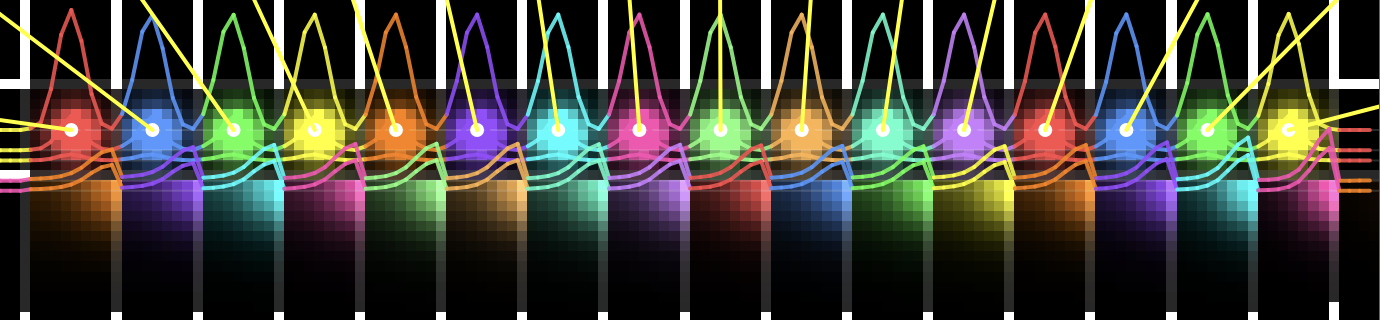
\includegraphics[width=\textwidth]{pictures/cable_domains.png}
\caption{The cable, relaxed. Sixteen sites along the axis, each with a kernel of charge $+3$, a core
domain of two electrons confined within $2.4\,a_0$, and one valence electron outside it. Colour
distinguishes domains; white verticals mark the free boundaries between neighbouring carriers, the
coloured curves are density profiles along the axis, and the yellow segments are net forces on the
kernels. Every boundary shown is an unknown of the minimisation.}
\label{fig:cable-domains}
\end{figure}

\paragraph{Case III: the same cable, carriers stiffened.}
The barrier is set less by the strength of the ion lattice than by whether the carriers bunch into
its wells: a carrier distribution that resisted being modulated would ride over the lattice, one
that does not resist locks to it. RealQM's free interface resists very little, and this is internal
to the construction --- a flat density is admissible on a free boundary at no cost, so redrawing an
interface between domains of equal density is free, and the only penalty on a \emph{modulated}
density is the gradient term, carrying the coefficient $\tfrac12$.

That coefficient is a standardisation rather than a constant of the theory, so the natural thing is
to ask how much the answer turns on it. Raising it from its physical $\tfrac12$, with ions,
standoff, geometry and mesh unchanged:

\begin{center}
\small
\begin{tabular}{@{}lrrrrr@{}}
\toprule
coefficient $c$ & $0.50$ & $0.60$ & $0.75$ & $0.90$ & $1.00$\\
\midrule
$\varepsilon_{\rm bulk}$ (meV) & $246$ & $159$ & $66$ & $20$ & $1$\\
in units of $kT$ & $9.5$ & $6.1$ & $2.6$ & $0.77$ & $0.04$\\
\bottomrule
\end{tabular}
\end{center}

\noindent The preferred registry is the same throughout --- the carriers sit on their own ion sites
at every value --- so what falls is the pinning itself and not merely its location. The barrier
crosses $kT$ between $c=0.75$ and $c=0.90$: a moderate stiffening, well short of doubling, brings
this cable out of the range where charge is held and into the range where thermal energy moves it.
The last entry should not be read as a value; one meV is below what the protocol resolves, and it
sits essentially at the coefficient where the barrier vanishes.

A barrier at $kT$ does not confine, so the pinning no longer holds and the charge is free to move.
What state the system is then in this measurement does not determine. It is not \emph{band}
conduction, since non-overlap admits no extended states for a band to be made of --- but that rules
out a mechanism, not a phenomenon, and whether the unpinned state would behave as a metal, as a
sliding charge lattice, or as something else is a question the instrument cannot reach. The
instrument measures a barrier; when the barrier goes, so does the instrument.

\paragraph{Case IV: a cubic lattice.}
The first three arrange their nuclei on a line. Hydrogen atoms can also be placed on a simple cubic
lattice at the same spacing in all three directions, and seventy-two of them --- three by three by
eight at $a=4.5\,a_0$, one electron per kernel, no core and no standoff --- make the fourth case.

What it settles is the binding. The lattice gives $-0.524$~Ha per atom against an eight-site chain's
$-0.453$, and below even the exact free atom's $-0.5$, because a domain in the lattice is a compact
cell of volume $a^3$ rather than a slab running out to the box face. It is also the
better-conditioned calculation, which was not expected of nine times the domains: its residual is
the smallest of any system here. A partition into compact cells is evidently closer to what the
functional would choose than one into elongated slabs, and the carrier density $n=1/a^3$ is exact
for this arrangement where the line of sites needs it as a convention.

What it does not settle is the barrier. The windowing above is not applied to it, so its difference
between the two registries carries the two junctions along with the bulk; on the chain that same
omission gave $642$~meV against the $394$ the windowed measurement returns. Its ${\approx}678$~meV
is therefore an upper estimate of a bulk quantity rather than one, and not comparable with the
windowed values. Supplying a real barrier means windowing the lattice as the chain and cable are
windowed, and scanning it.

\paragraph{A transport number the landscape settles by itself.}
A uniform field $F$ adds $-NeFd$ to the energy: it tilts the landscape and changes nothing else. The
field at which the barrier disappears is therefore a property of $E(d)$ alone --- no clock, no
temperature and no dissipation enter it. For a sinusoid of amplitude $V_0$ the steepest slope is
$\pi V_0/a$, so $F_{\rm th}=\pi V_0/ea$: $5.2$ and $3.2\times10^{9}$~V\,m$^{-1}$ for the chain and
the cable, and $2.6\times10^{8}$ for the stiffened cable. The first two are several times above the
dielectric strength of silica, ${\sim}10^{9}$~V\,m$^{-1}$, so those arrangements would break down
before they would slide --- which is what an insulator does. The stiffened cable is a factor of four
below it, so that one would slide first. The same separation that appears above as a barrier against
$kT$ appears here as a field against a breakdown strength, and neither statement needs a rate theory
to make it.

\paragraph{From a barrier to a conductivity.}
In the activated regime the corrugation is the activation energy in
$\sigma=(ne^2a^2\nu/kT)\,e^{-E_a/kT}$, where the exponential is the fraction of the time the system
is over the barrier and the prefactor $\nu=(1/2\pi)\sqrt{K/M}$ is how often it asks --- the
small-oscillation frequency of the collective coordinate, the charge pattern rocking against the ion
lattice. Since it is the sites that move, that rocking is a lattice vibration and $M$ is an ionic
mass. At $300$~K the chain and the cable give $0.1$ and $10$~S\,m$^{-1}$, bracketing intrinsic
germanium at $2$, and the attempt frequencies come out at $10^{12}$--$10^{13}$~Hz --- as energies
$h\nu$, $97$~meV for the hydrogen chain and $23$~meV for the cable, the former high because a proton
is light. Nothing was arranged to make that so, and it is the check that the mass entering $\nu$ is
the right kind of mass. Two orders of magnitude in $\sigma$ on a barrier ratio of $1.6$ is the
exponential at work: a difference of $148$~meV is $5.7\,kT$.

Three things enter from outside and should be named. The curvature $K$ is taken from an assumed
sinusoidal shape, which the scan shows to be too sharp, so the frequencies are overestimates even as
their scale is right. The mass is imported, because RealQM carries no masses --- the coefficient of
$|\nabla\psi_i|^2$ is a geometric scale, not $\hbar^2/2m$, which is exactly why it could be raised
above. And $n=1/a^3$ is a convention for turning a per-carrier barrier on a line of sites into a
bulk conductivity. What the framework supplies is the exponent.

\paragraph{What the cost of all this is.}
None of these systems is large, and it is worth saying why larger ones are not out of reach. The
electron--electron term omits $i=j$, so what each electron must be given is the potential of all the
\emph{others} --- the total less its own field, a different function for every $i$. A relaxation
step is therefore $N$ Poisson problems on the grid, and a multigrid solve costs work proportional to
the number of mesh points, so a step performs $N$ times the mesh of arithmetic. The single wave
function of textbook quantum mechanics, by contrast, lives on a $3N$-dimensional configuration space
and costs one grid raised to the power $N$. That difference, and not any detail of the arrangements
above, is why the question could be put at all.

\paragraph{Status.}
These barriers are rigid-slide values --- all carriers displaced together --- and that is the
expensive path. A cheaper one has one carrier advancing while the rest hold still, compressing the
domains ahead and expanding those behind. Every barrier here is therefore an upper bound and every
conductivity a lower bound, by a factor not yet determined, since the cheaper path has not been
computed. The lattice barrier is an estimate for the separate reason given above. What the framework
does not deliver in any regime is a resistive conductivity, whose relaxation time needs a current as
an object and irreversible dynamics: a minimisation over real densities has neither.

The instrument, at least, is sound: junction cancellation is exact by construction, linearity is
tested against a third window, translation by one spacing must return the same energy to the last
digit, and domains related by a symmetry must have equal eigenvalues. The full account, with the
convergence ladders, the controls and a link that reproduces every run in a browser, is in the
conduction article.

\section{Roadmap toward broader materials applications}\label{sec:material-roadmap}

The validated materials-science regime of Chapter~\ref{ch:condensed} (ionic crystals, molecular crystals where electrostatics dominates) is the working bottom of a larger ambition. We sketch what extensions would enable the framework to reach further into the materials-science landscape.

\paragraph{Metals.}
Metallic bonding is delocalised: conduction electrons spread across many atoms, and the non-overlapping unit-density picture of Level 3 has to be extended to accommodate this. This has now been examined directly rather than left as a prospect, and the outcome is that the extension is not optional but structural.

Section~\ref{sec:conduction} puts this to the test directly, and the outcome is more interesting than
a flat exclusion. A chain of one-valence-electron atoms does behave as a dielectric: each domain
carries exactly one electron by constraint, so no charge passes between sites and the polarisability
is extensive before anything is computed --- confirmed as $\alpha=7.6N$, flat to $1\%$ per atom.
But rearranging the same charge into a cable of ions surrounded by carriers drops the barrier into
the semiconductor range, and a moderate stiffening of the carriers takes it below $kT$.

Underneath the arithmetic one obstacle is genuinely structural: non-overlap makes the transfer
integral vanish identically. The transfer integral \emph{is} the overlap of neighbouring orbitals,
and there is none --- so the construction is not the Mott limit ($U\to\infty$ with $t\neq0$,
insulating but alive, conducting when doped) but the \emph{atomic limit}, where doping activates
nothing. \emph{Band} conduction is therefore absent in kind and not by degree: there are no extended
states for a band to be made of. That is a statement about a mechanism, and it does not by itself
decide whether the framework can produce conducting behaviour by another route --- which is the open
question Section~\ref{sec:conduction} ends on. A relaxed constraint permitting overlapping valence
territories would change the postulate rather than refine the implementation, and is one way out;
whether it is the only one is not established.

\paragraph{Semiconductors.}
Semiconductor physics as usually formulated depends on a small band gap and on the response of that gap to dopants, strain, and external fields --- and a band gap is a property of a band structure, which for the reason just given the Level-3 construction does not possess. That route is closed. Geometry the framework does reach: the tetrahedral and zincblende bonding topologies of Si, Ge and GaAs are within the angular splitting of the kernel valence sector, and cohesion, elastic response and defect energetics follow from it. And the \emph{transport} of the activated conductors turns out to be reachable by a different road, without a gap: Section~\ref{sec:conduction} measures a hopping barrier of ${\approx}240$~meV for a cable of ions, which is the activation energy such materials are characterised by. What remains outside is everything specifically tied to promotion across a gap --- intrinsic carrier statistics, the doping response through $t$, optical absorption edges.

\paragraph{Polymers and soft matter.}
Polymer chains and soft-matter systems are at the boundary between the molecular and the condensed regimes covered in Chapters~\ref{ch:folding} and~\ref{ch:condensed}. The Level-5 residue-level reduction of Chapter~\ref{ch:hierarchy} extends naturally to polymer monomer-level reductions, treating each monomer as an effective unit with appropriate electrostatic and steric profile.

\paragraph{Biological materials.}
Bones, shells, membranes, structural proteins (collagen, keratin), and biomineralisation are biological materials whose mechanical and electrostatic properties emerge from the interplay of atomic-scale interactions and supramolecular organisation. The hierarchy of Chapter~\ref{ch:hierarchy} reaches from atoms (Level 1) through proteins (Level 5) toward cellular structures (Level 6); biological materials lie in the Level-5 to Level-6 range, and the framework's reach into this regime is part of the vision Chapter~\ref{ch:hierarchy} sets out.

\paragraph{Electrochemistry and catalysis.}
Reactions at metal--solution interfaces (fuel cells, batteries, heterogeneous catalysis) are materials-science problems with an explicit chemistry component. RealQM's reactive chemistry handling (Chapter~\ref{ch:dimers}) combined with its Brownian-dynamics machinery (Chapter~\ref{ch:condensed}) puts the framework in a position to address such systems once the metal-extension above is in place.

\section{The framework's place in computational materials science}\label{sec:material-place}

We do not claim that RealQM is a replacement for DFT-MD or for empirical force fields in the materials-science workflow that has developed since the 1980s. Each tool has its regime; each tool has accuracy at a price the others do not pay.

\paragraph{What DFT-MD does that RealQM does not.}
\begin{itemize}
\item Chemical accuracy on covalent solids (silicon, diamond, transition-metal oxides) at well-validated functional level.
\item Band-structure and optical-property calculations through GW, BSE, and TD-DFT.
\item Dispersion correction (DFT-D3, MBD) at the post-DFT level for layered materials, molecular crystals, and biomolecules.
\item Decades of validated workflow: ground-state geometry, vibrational frequencies, elastic constants, thermal conductivity.
\end{itemize}

\paragraph{What empirical force fields do that RealQM does not.}
\begin{itemize}
\item Multi-microsecond molecular dynamics on protein-scale systems with known parameter sets.
\item Coarse-grained models (MARTINI, etc.) that reach mesoscale at low cost.
\item Reactive force fields (ReaxFF, REBO) for bond-breaking dynamics at scale.
\end{itemize}

\paragraph{What RealQM does that the others do not.}
\begin{itemize}
\item Ab initio condensed-phase phase transitions with no fitted parameters, at interactive cost on consumer hardware.
\item A unified framework that handles atoms, molecules, reactions, folding, and condensed phases from the same equation.
\item A regime-of-validity diagnostic (overshoot vs.\ missing dispersion) that the framework reports itself.
\item Interactive browser-based simulations suitable for pedagogy and rapid hypothesis exploration.
\item Real-space wave functions visualisable as charge densities, in continuity with Schr\"odinger's 1926 picture.
\end{itemize}

The framework's contribution to computational materials science is therefore complementary to the existing tools rather than competitive with them. It opens regimes that have been impractical (interactive condensed-phase exploration, real-time parameter sweeps on small materials systems) while leaving high-precision regimes to the established workflows.

\section{Significance: materials from a single principle}\label{sec:material-significance}

The most important statement of the materials chapter is structural rather than quantitative: \textbf{the same multiphase 3D continuum equation that handles a hydrogen atom (Chapter~\ref{ch:atoms}) handles a sodium-chloride crystal at finite temperature (Chapter~\ref{ch:condensed}), a protein folding under quantum-mechanical H-bond forces (Chapter~\ref{ch:folding}), and the helium-4 nucleus (Chapter~\ref{ch:nucleus}).} Materials science is, on this view, one application of a single variational principle that runs from femtometers to nanometers.

The accuracy of any one application varies with the regime --- chemistry at 1--10\%, condensed phases with calibrated overshoot, nuclear physics still exploratory --- but the underlying object is one equation. This is what is meant when the article and this book talk about the framework reaching scales beyond chemistry. Materials science is one of those scales; the rest of Part~III has worked through the others.

The next chapter takes the framework to Level 0 of the hierarchy, where the constituents are protons and electrons instead of electrons-around-a-kernel, and reports the validation of the same equation at the nuclear scale.

% --- End of Materials chapter ---


% --- Part IV: Foundations Revisited ---
\part{Foundations Revisited}\label{part:foundations-revisited}
\include{chapters3/ch13_stability_of_matter}
\include{chapters3/ch14_nucleus}
\include{chapters3/ch_nuclear_binding}
\include{chapters3/ch_nuclear_decay}

% --- Part V: Matter and Light ---
\part{Matter and Light}
\include{chapters3/ch15_sm_coupling}
\include{chapters3/ch_magnetism_spin}
\include{chapters3/ch16_excited_states}
\include{chapters3/ch17_molecular_radiation}
\include{chapters3/ch18_blackbody}
\include{chapters3/ch_time}
\include{chapters3/ch19_mystery_uncovered}

% --- Part VI: Connections ---
\part{Connections}
% ch_statistics chapter removed; the position on statistics is now stated in the
% Prologue (Coda: Dublin 1952), in the spirit of Schrödinger's 1952 Dublin remarks.
\include{chapters3/ch20_thermodynamics}
\include{chapters3/ch21_chemistry_vs_physics}
\include{chapters3/ch_philosophy}
\include{chapters3/ch_ontology}
\include{chapters3/ch_relativity}
\include{chapters3/ch_cosmology}
\chapter{The Human--AI Collaboration}\label{ch:collab}
\index{Anthropic, Claude}\index{Claude (AI)}\index{Body and Soul programme}\index{human-AI collaboration}

\begin{quote}
\itshape If we are still going to have to put up with these damned quantum jumps, I am sorry that I ever had anything to do with quantum mechanics.\\
\normalfont\hfill --- E.~Schr\"odinger to N.~Bohr, 1926.
\end{quote}
\bigskip

The mathematical reformulation of Chapter~\ref{ch:equation} and the hierarchy of Levels 1--4 in Chapter~\ref{ch:hierarchy} are the work of the human author. They predate the AI collaboration and have been developed over a decade of independent work. The author also wrote the initial p5.js prototype simulations that established the numerical core --- real-space grid, imaginary-time propagation, Poisson solver, basic visualisation --- used as the starting point for the WebGPU implementation.

The full WebGPU port, the validation suite reported in Part~III, the systematic kernel-architecture sweeps, and the curated public Gallery were developed from those starting templates through extended collaboration with \textbf{Claude}, an AI code assistant produced by Anthropic. We document the pattern of the collaboration in this chapter because we believe it is a worth-reporting example of how a single mathematical mind can produce research-grade interactive scientific software with an AI engineering partner, at a scale otherwise requiring a programming team.

This chapter is not about the philosophy of human--AI cooperation in general. It is about a specific working relationship that produced specific results, with a specific division of labour, over a specific period of time. We report what happened, what worked, and where the AI's interpretations had to be corrected by the human.

\section{Precursor: the Body and Soul project}\label{sec:body-and-soul}

The Mind--AI cooperation described in this chapter did not begin in 2025. It is the most recent stage of a much longer programme by the author and his collaborators, known as \textbf{Body and Soul}, that has been running for more than two decades. Body and Soul is a constructive--computational reformulation of applied mathematics --- calculus, differential equations, fluid mechanics, solid mechanics, electromagnetics --- aimed at restoring the constructive character that mathematics had before the 20th-century formalist turn made it largely non-computational at the undergraduate level. The series of textbooks and monographs published under that banner~\cite{BodyAndSoulI,BodyAndSoulII,BodyAndSoulIII,BodyAndSoulIV,BodyAndSoulV} works through the standard curriculum of applied mathematics in a way in which every concept is realised numerically and every theorem is paired with an algorithm that produces a finite computable answer.

The first three volumes (Eriksson, Estep, Johnson, Springer 2004) carried calculus and differential equations through the constructive reformulation. The fourth volume, \emph{Computational Turbulent Incompressible Flow} (Hoffman and Johnson, Springer 2007), took the same methodology into the regime of turbulent fluid mechanics --- arguably the hardest classical PDE problem in applied mathematics --- and produced working algorithms for the Navier--Stokes equations at high Reynolds number, paired with mathematical analysis of the Clay Millennium open problem on the regularity of weak solutions. The Hoffman--Johnson collaboration that produced Volume 4 is, in the framing of this chapter, the immediate human-collaboration precursor to the human--AI collaboration that has produced the present quantum-mechanics volume: in both cases a single mathematical agenda was carried through to a complete computational implementation by a small team working across years.

The fifth volume, \emph{Computational Thermodynamics} (Johnson, in preparation), is currently a draft in development. It carries the constructive--computational reformulation into thermodynamics, with the same characteristic insistence that every concept be paired with a computable algorithm. Together with the present quantum-mechanics volume, it represents the two most recent extensions of the Body and Soul programme into regimes that have classically resisted the constructive treatment: thermodynamics, where statistical-mechanical language has dominated since Boltzmann, and quantum mechanics, where the probabilistic Born interpretation has dominated since 1926. The Body and Soul approach to both is the same: replace the probabilistic/statistical interpretive layer with a deterministic real-space formulation whose computations are directly checkable against observation.

A \textbf{planned volume on quantum mechanics} has been part of the Body and Soul agenda since the early stages of the project. Quantum mechanics is the natural next target for the constructive--computational reformulation, for the same reason it was the target of Dirac's 1929 statement: the underlying physical laws are known, and the obstacle is making the equations tractable. The Body and Soul approach to such an obstacle has always been to write the algorithm that produces the answer, then verify against observation. For quantum mechanics, however, the algorithm-producing step was not feasible for a single mathematical mind to carry through to a complete validated implementation: the configuration-space scaling made the standard $3N$-dimensional formulation intractable, and the alternative real-space formulation required a working implementation of the kind that previously required a programming team.

\textbf{The present book is the quantum-mechanics volume of Body and Soul, made possible by the Mind--AI cooperation.} The two-part contribution mirrors this: the mathematical reformulation (Chapter~\ref{ch:equation}) and the hierarchy of reductions (Chapter~\ref{ch:hierarchy}) extend the Body and Soul programme into quantum chemistry; the implementation, validation suite, and Gallery (Parts~II--III) realise the algorithmic ambition that the earlier solo work could not reach. The structural continuity is direct: each volume of Body and Soul replaces formalist abstractions with computable objects; this volume replaces the configuration-space wave function with non-overlapping unit densities on physical 3D space, and replaces the unsolvable many-body Schr\"odinger equation with a free-boundary variational problem that can be solved on a laptop GPU.

The chapter's opening epigraph --- Schr\"odinger's 1926 ``damned quantum jumps'' remark to Bohr --- records the discomfort the founder felt with the direction the field took immediately after his 1926 wave equation. The RealQM volume of Body and Soul is, among other things, a long-overdue answer to that complaint: a formulation in which the wave function is a charge density on physical space, and there are no damned quantum jumps.

\paragraph{Why the QM volume waited.}
Earlier Body and Soul volumes were produced by the author and his collaborators on a timescale of several years per volume, through close mathematical work and conventional programming. The QM volume was sketched in lectures, blog posts, and partial drafts (including the 2017 draft from which the prel-book chapters of \texttt{RealQuantum/} are taken) but did not reach a complete implementation. The bottleneck was not the mathematics --- the multiphase reformulation has been stable in the author's notes for over a decade --- but the implementation. A working WebGPU port of the variational solver, with a full validation suite and a public Gallery, was not within reach of solo programming on any reasonable timescale.

The AI partner closed that gap. The same person who had carried the earlier volumes to completion through years of solo work could now reach the implementation in months by working with Claude. The Body and Soul programme therefore acquired its long-planned QM volume not by changing the underlying mathematical reformulation --- the reformulation is the author's, and predates the AI collaboration by more than a decade --- but by making the implementation tractable for a single mathematical mind.

\paragraph{Continuity of method, change of cost structure.}
The methodological continuity from earlier Body and Soul volumes to this one is straightforward to state:
\begin{itemize}
\item Every quantitative claim in this book corresponds to a runnable simulation in the Gallery (the Appendix).
\item Every architectural choice is checked against observation rather than against an analytic limit.
\item Every limitation in Chapter~\ref{ch:limits} is identified empirically rather than reasoned about abstractly.
\item Every reduction in the hierarchy of Chapter~\ref{ch:hierarchy} is calibrated against the previous level numerically.
\end{itemize}
What changed is the cost of executing this method on quantum mechanics. Body and Soul on calculus or fluid mechanics could be done by a small team over years; Body and Soul on quantum mechanics, with the multiphase formulation, became achievable for one author plus AI partner over months.

The framing of this chapter --- \emph{mathematical mind + AI engineering partner}, discussed in Section~\ref{sec:framing} --- is therefore the natural extension of the Body and Soul model to a problem whose implementation cost had previously placed it out of reach. The book is the QM volume of Body and Soul, and the chapter you are reading is the working note on how the implementation cost was overcome.

\section{Division of labour}\label{sec:division}

The mathematics, the theory, the chemical questions, and the standards for what counts as evidence are the human's. The implementation, the systematic exploration, the speed of code generation, and the breadth of parameter sweeps are the AI's. Neither could have produced the work reported in this book alone in any reasonable timeframe.

\paragraph{What the human brought.}
\begin{itemize}
\item The multiphase 3D reformulation of the $N$-electron Schr\"odinger equation (Chapter~\ref{ch:equation}).
\item The Bernoulli free-boundary condition as the closing condition of the variational problem.
\item The hierarchy of reductions, Levels 1--4 (Chapter~\ref{ch:hierarchy}).
\item The initial p5.js prototype simulations that established the numerical core.
\item The chemical intuition for which architectures to try on which molecules.
\item The mathematical standards for what counts as a validation result.
\item The connection to historical foundations (Dirac, Schr\"odinger 1926 letter, Solvay 1927).
\item The interpretation of results in the broader context of the chemistry-versus-physics debate.
\end{itemize}

\paragraph{What the AI brought.}
\begin{itemize}
\item Translation of mathematical and chemical questions into runnable simulations.
\item Real-time bug identification in the code.
\item Systematic parameter sweeps with results tabulated and analysed.
\item Drafting of candidate Gallery cards and validation summaries.
\item Challenging claims that did not survive scrutiny.
\item The full WebGPU implementation including the WGSL compute shaders.
\item The infrastructure of the validation suite and the public Gallery.
\end{itemize}

The division was not rigid. The human wrote code; the AI proposed theoretical refinements that survived the human's review; both iterated on the framing of the results. What was rigid was the standard: a claim entered the manuscript or the Gallery only after both human and AI agreed it was supported by the evidence.

\section{The working pattern}\label{sec:working-pattern}

The interaction was iterative and surprisingly productive. A representative cycle:

\begin{itemize}
\item \textbf{9:00.} Human asks: ``What if the model uses $Z = 2$ instead of $Z = 4$ for carbon?''
\item \textbf{9:05.} AI produces a working scan file in which the C kernel is parameterised by $Z$ and the user can sweep it.
\item \textbf{9:30.} Partial results from a first sweep at three values of $r_c$ and two values of $Z$.
\item \textbf{10:00.} Full sweep table with energies at the experimental bond length and at twice that.
\item \textbf{10:30.} Refined analysis incorporating the latest data; identification of which $(Z, r_c)$ pair gives the best match for CH$_4$.
\end{itemize}
Across many such cycles --- spanning weeks to months on each major chapter of the validation --- the table reported in Chapter~\ref{ch:hydrides} was assembled. The same pattern produced the S66 dimer geometries, the protein-folding results, and the condensed-phase calibration.

\paragraph{Why the speed matters.}
The cost of an iteration on a question like ``does this kernel architecture match the chemistry?'' is normally measured in days or weeks: write the code, compile it, run it, parse the output, iterate. With the AI partner, the iteration cost dropped to minutes. The accessible space of questions grew correspondingly. Many of the systematic sweeps reported in Chapters~\ref{ch:atoms}--\ref{ch:condensed} would not have been undertaken at all if the iteration cost had remained at the pre-collaboration scale; the questions were possible because the answers were cheap.

\paragraph{Why the breadth matters.}
A single researcher exploring a parameter space typically tests a small number of points based on intuition and reasoning. The AI partner extends this by running systematic sweeps that cover the parameter space densely, identify trends, and surface results that intuition would not have predicted. Several of the Level-3 architecture results in this book --- including the periodic-table sweep of $r_c$ across groups 1, 2, 14, and 16 --- came out of such systematic sweeps. The human posed the question; the AI ran the experiments densely enough that the pattern became visible.

\section{Where the AI was wrong}\label{sec:where-wrong}

We record honestly where the AI's interpretations needed correction. The pattern is consistent enough to be worth describing as a working note for others contemplating similar collaborations.

\paragraph{Premature convergence claims.}
Several times the AI prematurely concluded that a result was ``within $X\%$ of experiment'' before convergence had been confirmed. The relaxation algorithm of Chapter~\ref{ch:relaxation} has multiple coupled convergence indicators (total energy, Hartree residual, boundary motion), and the AI sometimes reported an apparently stable energy before the boundary update had finished settling, leading to numbers that drifted by a few percent on continued iteration. In each case the human pushed back, the AI re-ran the calculation to deeper convergence, and the reported number was revised.

\paragraph{Over-confident regime extrapolation.}
Early in the collaboration the AI was inclined to extrapolate a successful result into regimes where it had not been tested. A working architecture for one molecule was sometimes proposed as a general method for an entire class before the class had been swept. The human's response was to demand the sweep before accepting the generalisation; this discipline shaped Chapter~\ref{ch:hydrides}'s structure, where every group was swept rather than extrapolated from one example.

\paragraph{Insufficient skepticism on accuracy claims.}
The model's accuracy at $\sim$3--9\% on bond energies was sometimes overstated as ``chemical accuracy'' in early drafts. Chemical accuracy is $\sim$1 kcal/mol; 3--9\% of $\sim$300~kcal/mol is $\sim$10--30 kcal/mol, an order of magnitude larger. The human enforced the distinction; the final accuracy claims in this book are more honest than the earlier AI-drafted versions were.

\paragraph{Status of the corrections.}
The Gallery's ``Assessment by Claude'' card reflects this history. Its caveats were rewritten more than once during the project as evidence accumulated and as overstated claims were retracted. The card is not a clean record of confident conclusions; it is a record of the back-and-forth that produced the conclusions. We consider this part of the contribution rather than an embarrassment to be hidden: \emph{the corrections are how the work was done}.

\section{The framing: mathematical mind + AI engineering partner}\label{sec:framing}

The right framing for the collaboration is \textbf{mathematical mind + AI engineering partner}. The human supplies the theory, the questions, the chemical intuition, and the standards for what counts as evidence. The AI supplies the implementation, the systematic exploration, and the speed.

This is not the same as ``the AI did most of the work.'' The AI did not invent the multiphase 3D reformulation, did not derive the Bernoulli free-boundary condition, did not propose the hierarchy of Levels 1--4, did not connect the work to Dirac's 1929 position. These are the work of the human, accumulated over a decade of independent research. What the AI did was take those mathematical ideas and the initial p5.js prototypes, and build them out into a full implementation with a complete validation suite, in a fraction of the time it would have taken a programming team.

\paragraph{What the AI cannot do.}
The AI cannot evaluate whether a chemical result is surprising. It cannot judge which questions are worth asking. It cannot connect a numerical finding to a broader theoretical claim. It cannot decide what counts as a satisfying explanation. In every case where these judgements were called for, the human made the judgement; the AI implemented the consequence.

\paragraph{What the human cannot do alone.}
A single researcher cannot, in any reasonable timeframe, write 8000 lines of WebGPU compute shaders with a complete validation suite, a public Gallery, systematic kernel-architecture sweeps across multiple periodic-table groups, and condensed-phase calibration across three crystal systems. The breadth of the validation in Part~III is what the AI partner made possible.

The combination is what produced the work. Either alone --- human without AI, or AI without human --- would have produced less, slower, and in a different form.

\section{Can an AI clean up a hundred years of patchwork?}\label{sec:ai-patchwork}

The collaboration described above raises a question larger than this project. If a mathematical mind
paired with an AI partner can build and validate a framework in months, what should we expect such
pairings to do to quantum chemistry generally? The question divides in two, and the two halves have
different answers --- which is itself the interesting result.

\paragraph{First: can it clean up the standard patchwork?} Partly, and the work is already under
way. Machine-learned exchange--correlation functionals exist and repair failure cases that defeated
hand-built ones. Neural-network trial functions go further and dispense with functionals altogether,
using a network as the ansatz in a variational calculation: no functional is named, the result is a
genuine upper bound, and on small systems the accuracy is competitive with the best conventional
methods. Anyone who says machine learning has added nothing here is not looking.

But notice what this does. It \emph{compresses} the patchwork: one learned object replaces many
hand-crafted ones. It does not remove the reason the patchwork was needed, because the
$3N$-dimensional problem is untouched and any method that scales remains an ansatz or a functional.
A learned functional is fitted --- fitted better, on more data, with more care, but fitted. A
hundred small fits become one large fit, and the argument of Chapter~\ref{ch:precision} applies to
the one exactly as it applied to the hundred: there is still an ingredient standing between the
equation and the number, so the equation still cannot fail.

The trade also has a cost that is rarely counted. The patchwork is at least \emph{legible}. Each
approximation carries a name, a published derivation, a known failure mode, and a user who can say
why it was chosen. A learned functional carries none of that. One exchanges a hundred inspectable
approximations for a single approximation that cannot be inspected, and buys no exposure to
refutation in return. Cleaning up, here, is compression and not derivation.

\paragraph{Second: can it realise a computable model?} Here the answer is yes, for a dull reason
that turns out to matter. The bottleneck of this programme was never ideas; it was the labour of
computing consequences and checking them --- building the solvers, imposing the right conditions at
the free boundaries, running the grid ladders, comparing against exact values and against
measurement. That labour is precisely what has become cheap. Constructions that would each have
taken weeks take hours, so claims can be confirmed and, more usefully, killed at a rate that was not
previously available.

The condition is the one Section~\ref{sec:where-wrong} records at this project's own expense: every
claim must be pinned to something outside the calculation that produced it --- an exact value, a
measurement, a halved grid, a number computed by different code. Fluent output is not evidence, and
the failures do not announce themselves. But those anchors are available here, and not by luck. They
are available \emph{because} the model is computable and has nothing left to choose.

\paragraph{Why the two answers differ.} An AI accelerates whatever it is applied to. Applied to a
theory whose usable versions are all parameterised, it accelerates parameterisation: better
functionals, better surrogates, better fits. That is valuable engineering and it tells us nothing
about whether the theory is right, because nothing in it was ever at risk. Applied to a theory that
can be computed outright, it produces verdicts --- and some of them will be unfavourable, which is
the point and not a drawback. Several of this book's own claims were withdrawn that way.

So the collaboration does not make RealQM correct. It makes RealQM \emph{decidable in practice}. A
theory that can be decided is worth more than one that cannot, whichever way the decision goes, and
that is the sense in which the tooling of the last few years bears on a hundred-year-old question.

\section{The collaboration as part of the contribution}\label{sec:collab-contribution}

We report the collaboration as part of the contribution because we believe it has implications for how research-grade scientific software gets built going forward. The pattern --- a single mathematical mind paired with an AI engineering partner, producing in months what previously required a programming team and several years --- is not specific to this project. It is a working pattern that we expect to see repeated, particularly in fields where the underlying mathematics is mature but the implementation has been a bottleneck.

\paragraph{Implications for scientific software.}
The traditional model of scientific software --- large packages developed over decades by teams of dozens, with the code becoming progressively harder to modify --- may not be the only viable model. The RealQM implementation is approximately 8000 lines, built in months, modifiable by the same person who wrote it. The scale compression matters; software at this scale can be re-implemented, ported to new hardware, or radically refactored on a timescale of weeks. The maintenance overhead that constrains large packages is largely absent.

\paragraph{Implications for who can do computational science.}
The collaboration model also shifts the entry barrier. Producing a working WebGPU implementation of a quantum chemistry framework, with a complete validation suite, no longer requires a research group with dedicated software engineers. It requires one mathematical mind and one AI partner. This expands the population of people who can contribute computational tools to chemistry; the pattern is not specific to this author.

\paragraph{What is reported here.}
We do not claim the collaboration is the central contribution; the central contributions are the mathematical reformulation and the validation reported in Parts~I--IV. But the collaboration is part of how the science came into existence, and we report it as such. Readers contemplating similar collaborations will find the pattern described in this chapter --- division of labour, working iteration, recorded corrections, the framing of mathematical mind + AI engineering partner --- a useful template.

% --- End of Chapter 17 ---

\chapter{What ``Exact'' Means}\label{ch:precision}
\index{exactness}\index{fitted model}\index{Lamb shift}\index{anomalous magnetic moment}\index{atomic units}\index{Planck's constant!as a fitted scale}

\begin{quote}
\itshape A fitted model is exact in the aspect it was fitted to.
\end{quote}
\bigskip

Every objection this book has met comes back to one comparison. Standard quantum mechanics is said
to be exact and merely uncomputable; RealQM computes but agrees with measurement only to a few per
cent. Put that way the matter is settled before it is examined. This chapter examines it, and the
sentence above is the whole of the argument. Exactness in the aspect a model was fitted to is
automatic --- it was arranged, and it carries no information. What a model does \emph{outside} its
fit is the only thing that can fail, and therefore the only thing that is evidence.

\section{The premise}\label{sec:prec-premise}

The claim that organises every introduction to the subject is that the Schr\"odinger equation
solves hydrogen exactly. For one electron about a fixed point charge,
\begin{equation}
-\tfrac12\nabla^2\psi - \frac{1}{r}\,\psi = E\psi,
\label{eq:prec-schrH}
\end{equation}
with ground state $E=-\tfrac12$ in atomic units, $13.605693$~eV, and spectrum $E_n = -1/2n^2$
reproducing the Balmer series. The agreement was decisive in 1926 and remains the reason the
equation is believed. The question is what that agreement establishes --- and to answer it one must
ask where the two terms in \eqref{eq:prec-schrH} came from, because they did not come from the same
place.

\section{Where the form came from}\label{sec:prec-form}

\paragraph{The potential is not ad hoc.}
The term $-1/r$ is Coulomb's law, and it enters \eqref{eq:prec-schrH} already established. It was
measured by Coulomb in 1785 on a torsion balance at macroscopic separations, in experiments that
knew nothing of atoms or of spectra, and the inverse-square form has since been confirmed to high
precision in settings unrelated to the hydrogen atom. It arrives with no freedom: no exponent to
select, no prefactor to tune, nothing adjusted to atomic measurements. Whatever fitting went into
\eqref{eq:prec-schrH}, the Coulomb term is not where it happened.

\paragraph{The kinetic term is.}
The operator $-\tfrac12\nabla^2$ has no comparable standing. Nothing in electrostatics or mechanics
requires the quadratic form $T[\psi] = \tfrac12\int|\nabla\psi|^2$, and it was not derived from
anything prior. Schr\"odinger reached it by analogy --- with Hamilton--Jacobi theory and with de
Broglie's relation --- and an analogy is not a derivation. The decisive detail is what happened to
the alternative: he wrote a relativistic wave equation first, found that its eigenvalues gave the
wrong fine structure for hydrogen, and set it aside in favour of the non-relativistic form, which
gave the right gross spectrum. The surviving operator is the one that produced the observed levels.
It was selected \emph{by} its spectrum.

So the two ingredients have opposite status. One carries independent empirical support obtained
without reference to atoms. The other was chosen because its eigenvalues came out as the ones
already on the table.

\paragraph{What was on the table.}
The pattern was known before the equation existed: Balmer wrote his formula for the visible
hydrogen lines in 1885 and Rydberg generalised it in 1888, both purely empirically, the lines going
as differences of $1/n^2$. Equation~\eqref{eq:prec-schrH} was accepted because it returns exactly
this. The $1/n^2$ pattern is a consequence of the equation, but the equation is a consequence of
the pattern.

The famous $-0.500000$ has a second and separate issue: its digits are not an outcome. The
coefficient $\tfrac12$, and with it a ground state at exactly $-\tfrac12$, is a statement about
units --- atomic units are \emph{defined} so that this is the number. Converting it into anything
measurable needs a bridge from atomic energy to the energy of light, and that bridge is Planck's
constant, through $\Delta E = h\nu$. But $h$ --- equivalently $R_\infty$, since the Hartree is
$2R_\infty h c$ --- is itself fixed by spectroscopy, and the hydrogen spectrum is among the
measurements that fix it. The scale is read off the spectrum and then put back into it.

In the narrow sense the equation has no adjustable parameter: given $\hbar$, $m_e$ and $e$ the
ground state follows. In the sense that matters for the word \emph{exact}, it is a model of simple
form whose form and whose scale were both selected to fit one body of data --- and it is that body
of data which is then presented as its triumph.

\section{Outside the fit}\label{sec:prec-outside}

For hydrogen the fitted aspect is the bound-state spectrum: the $1/n^2$ pattern and, through $h$,
its scale. Exactness there is free. The first genuinely unfitted predictions are close at hand, and
the equation gets them wrong.

One candidate failure must be set aside first, because it is not the equation's. The nucleus moves,
and \eqref{eq:prec-schrH} holds it fixed --- but that is a shortcoming of how the equation has been
\emph{applied}, not of the equation. Written for two bodies it separates exactly into
centre-of-mass and relative motion, and the relative part returns the hydrogenic spectrum with the
reduced mass in place of $m_e$, giving $13.598287$~eV. That is the equation's own answer, obtained
exactly. Charging the proton's motion against \eqref{eq:prec-schrH} would repeat precisely the
misattribution this chapter is about.

What remains cannot be dismissed that way. Against the measured $13.598435$~eV the residual is
$0.000147$~eV, or $1.1\times10^{-5}$ relative --- the relativistic and radiative physics the
equation does not contain. Five significant figures, not infinitely many. And the spectrum fails
more sharply, qualitatively rather than numerically: \eqref{eq:prec-schrH} makes $2s$ and $2p$
exactly degenerate, and they are not. The splitting is $1057.845$~MHz, the Lamb
shift~\cite{LambRetherford}, whose discovery in 1947 initiated renormalised quantum
electrodynamics. Here the equation does not return
a slightly wrong number; it returns zero where there is an effect.

So the equation said to be exact for hydrogen is the leading term of an expansion, completed by
Dirac and by quantum electrodynamics. None of this is news to atomic physics. It is a correction to
what the hydrogen case is taken to establish.

\section{The step that is not justified}\label{sec:prec-step}

For $N$ electrons the equation is written in $3N$ dimensions with $\Psi$ antisymmetric. This is a
separate postulate. It is not derived from \eqref{eq:prec-schrH}, and \eqref{eq:prec-schrH} does not
determine it: a one-electron equation fixes nothing about the dimension of the space the
many-electron problem is posed in. Antisymmetry is a further addition again, since the bare
equation is content with symmetric solutions and with them predicts the wrong periodic table.

The inductive support offered for the $3N$ postulate is the hydrogen case --- where, by
Section~\ref{sec:prec-form}, the exactness is in the fitted aspect and therefore empty, and where,
by Section~\ref{sec:prec-outside}, the unfitted predictions fail. That is a thin foundation for a
claim of exactness at every $N$.

\section{The showcase, and what it shows}\label{sec:prec-ae}

The claim examined here is usually made in the form Feynman gave it, and it is worth having in his
words. Having quoted the electron's magnetic moment as $1.00115965221$ from experiment against
$1.00115965246$ from theory, he writes~\cite[ch.~1]{FeynmanQED}:
\begin{quote}
\itshape At the present time I can proudly say that there is no significant difference between
experiment and theory! \dots\ To give you a feeling for the accuracy of these numbers, it comes out
something like this: If you were to measure the distance from Los Angeles to New York to this
accuracy, it would be exact to the thickness of a human hair.
\end{quote}
The figures have improved since --- the moment is now measured to $0.13$ parts per
trillion~\cite{Fan2023} and agrees with the calculated series~\cite{Aoyama2019} at about one part
in $10^{12}$ --- and this is the evidence meant whenever it is said that no observation has ever
been found to disagree with quantum mechanics. The description of it as the most precisely tested
prediction in science is fair; the inference usually drawn from it is not.

Notice first what Feynman is careful to say, and about what. His claim is about \emph{quantum
electrodynamics}, which he names in the same breath, and the number he selects is a one-particle
quantity. That is precisely the distinction this section turns on, and the canonical source for the
precision claim already observes it.

The quantity is one-particle. It concerns a single electron's coupling to the quantised
electromagnetic vacuum, computed as a perturbative series in $\alpha$ within quantum
electrodynamics. It involves no many-electron wavefunction, no antisymmetry among several
electrons, no $3N$-dimensional equation. It is overwhelming evidence that QED describes the vacuum
coupling of one charge, and it is not evidence about the many-electron equation; offering it in
support confuses two different theories that happen to share a Lagrangian. Two further points
belong with it: the comparison requires $\alpha$, whose most precise determinations now come either
from the moment itself or from atom-recoil measurements that have at times disagreed at the level
of the comparison, so part of the agreement is internal rather than independent --- and the
precision is a property of the observable, not of the theory's reach. Twelve digits on a vacuum
quantity coexists with no ability to state an error bar on a hundred-electron molecule.

The last point is not a private complaint of this book's. Leggett, reviewing what has actually been
tested, opens from the same observation~\cite[p.~R415]{Leggett2002}:
\begin{quote}
\itshape Despite this enormous range of applications, however, there is a sense in which we can say
that the region of the whole parameter space over which the validity of QM has been directly tested
is still rather modest.
\end{quote}
His concern is length scale and the size of superposed objects rather than electron count, but the
shape of the argument is the one made here: a theory can be confirmed to many digits inside a
narrow region and remain untested across most of the range over which it is nonetheless assumed.

\section{Where the equation can be solved}\label{sec:prec-solve}

For an equation advertised as exact for every $N$, the question that decides what the advertisement
is worth is: for which $N$ has it been \emph{solved}? Not approximated --- solved, to an accuracy
the equation itself controls.

The answer is two, three, and with effort four. Helium is known to some twenty digits and H$_2$ to
twelve, by explicitly correlated expansions in the interelectronic distances. These are not
truncations of a general procedure that merely becomes expensive; they are constructions built for
a handful of particles, and they do not continue.

Past that the equation is not solved. It is projected onto a finite basis and the projection is
solved instead. Full configuration interaction reaches of order ten electrons in a basis too small
to be the answer, at a cost that grows factorially, and the remaining error is the basis's rather
than the equation's --- not quantifiable against the exact solution, because the exact solution is
what is missing. Beyond ten electrons the working methods are different theories: coupled-cluster
at a chosen truncation, or density functionals carrying parameters fitted to measured data, the
latter having given up the wavefunction altogether. They are effective and they are what chemistry
uses. Neither is the Schr\"odinger equation. For a protein there is no number of any kind.

There is a further turn, and it bears on how this book's per-cent figures should be read. The
numbers a competing model is scored against are themselves largely computed. The $-2.903724$ for
helium is not a measurement: it is the solution of the nonrelativistic Schr\"odinger equation at
infinite nuclear mass, obtained by a purpose-built expansion --- the equation under test supplying
its own benchmark. What is measured is the two ionization energies, and summing the NIST values
gives $-2.903386$~Ha; the remaining $0.00034$~Ha is \emph{removed by calculation}, being the
relativistic, QED and nuclear-motion content the measurement contains and the benchmark must not.
They part company in the fourth decimal and theory supplies the difference. For atoms generally the
reference energies are explicit composites of experiment and \emph{ab initio} calculation, computed
outright past argon~\cite{Chakravorty}, because a nonrelativistic stationary-nucleus total
electronic energy is not an observable --- no instrument reads one. The composites are accurate and
this does not impugn them. It does mean that ``agrees with the exact value to $n$ per cent'' states
a distance from a construction that already contains the theory under test, which is why
Chapter~\ref{ch:atoms} rests its case on observables of another kind --- ionization energies,
geometry, shell radii, ordering.

So the equation is exact for all $N$ and solvable for $N$ of about three. An exactness testable
only where a bespoke method happens to exist, and replaced by fitted models everywhere else, has no
content at the sizes chemistry and biology are made of.

\paragraph{Why the claim of universal agreement is nearly empty.}
This is the point at which the two halves of the standard position --- \emph{exact} and
\emph{uncomputable} --- turn out to undercut one another, and it is worth stating bluntly. A
disagreement with observation requires a prediction to disagree with. Past three or four electrons
the $3N$-dimensional equation yields no number at all; the numbers come from truncations and from fitted
functionals. So for almost all of chemistry there is nothing for an experiment to contradict, and
the celebrated record of never having been contradicted is, at those sizes, not a record of success
but a record of \emph{absence of exposure}.

The practice follows accordingly, and consistently. When a computed result does fail --- dispersion
missing, a barrier wrong, a spin state out of order --- the failure is charged to the functional or
to the basis and is repaired by adjusting those, never charged to the equation. That attribution is
not dishonest; it is correct, because the equation was never evaluated and so cannot be what failed.
But it means no observation can reach the equation at all. Uncomputability places it beyond
refutation, and what is beyond refutation is equally beyond confirmation: the unbroken agreement is
a property of the arrangement, not a finding about nature.

So the claim retains content exactly where computation is possible --- hydrogen, helium, the
one-particle vacuum quantity of Section~\ref{sec:prec-ae} --- which is also where the form was fitted
and where the showcase sits. Everywhere else it is the empty statement that a theory which makes no
checkable prediction has never been caught out. This is the same structure as the principle in
Section~\ref{sec:prec-form}, arrived at from the other side: there, exactness in the fitted aspect
carried no information because it was arranged; here, agreement carries no information because
nothing was risked.


\section{What the comparison is about}\label{sec:prec-conclusion}

The two models are both postulates. Both generalise Coulomb interaction and a chosen kinetic form
to many electrons, in different ways, and neither generalisation is derived. They differ in what
can be done with them.

One is exact in a limit nobody can compute, misses by $1.1\times10^{-5}$ and by a whole splitting
in the one case it solves exactly, achieves extraordinary precision for two and three electrons by
methods that do not scale, and offers no error bar at all past ten. The other is exact nowhere,
agrees with measurement to a few per cent, and does so at every size from one electron to ten
thousand, in three dimensions, at linear cost.

The first is more accurate wherever it can be evaluated. The second is \emph{answerable} wherever
matter exists. A theory whose error is knowable and roughly constant can be held to account at
every scale; a theory whose error is unquantifiable past three electrons can be held to account
only there. Which property matters more depends on what one wants a model of matter for --- and
that is a question about scope, which is a legitimate scientific question, rather than a question
about precision, which the twelve digits have already settled in a domain where nobody disputes
them.

Chapter~\ref{ch:h2} makes the same point with numbers on the one system where both models can be
pushed to convergence: the two RealQM constructions available at $N=2$ bracket the exact energies
of He and H$_2$ from either side, and the few per cent they leave is the same few per cent the model
carries at ten thousand electrons, for the same reason.

% --- End of chapter ---

\chapter{Limitations}\label{ch:limits}
\index{regime mapping}\index{anions (limitations)}\index{dispersion!van der Waals}\index{Pauli repulsion (short-range)}\index{blind folding}\index{chemical accuracy}

\begin{quote}
\itshape With very few exceptions (such as Einstein and Laue) all the rest of the theoretical physicists were unadulterated asses and I was the only sane person left. [\ldots] The one great dilemma that ails us [\ldots] day and night is the wave--particle dilemma [\ldots] So unable is the good average physicist to believe that any sound person could refuse to accept the Copenhagen oracle.\\
\normalfont\hfill --- E.~Schr\"odinger to J.~L.~Synge, 1959.
\end{quote}
\bigskip

A serious theory of matter has to say what it cannot currently do as well as what it can. This chapter is an honest accounting of the boundary of RealQM's regime: where the framework works cleanly, where it works partially, and where the present formulation has not yet been extended. The accounting is empirical --- derived from systematic testing over a wide range of systems --- rather than a theoretical statement about which regimes the formulation must in principle handle. The framework's actual current regime is what the tests have shown it to be, and the tests have shown that some regimes lie beyond present reach.

We organise the chapter around three categories: the working regime (where Parts~II and III have validated the framework), the partial regime (where the framework works only with constraints or only on geometry, not energetics), and \textbf{current limitations} (where the framework at the present stage of development does not yet handle the relevant physics, but where an extension --- explicit solvent, correlation, longer-range interactions --- is the natural next step). We close with the structural reasons for each limitation and an honest comparison to standard quantum chemistry on its terms.

\section{The working regime}\label{sec:working-regime}

These are the systems and phenomena where RealQM has been shown to reproduce experiment within a defined accuracy.

\paragraph{Atomic and molecular energetics, Levels 1--3.}
\begin{itemize}
\item Total atomic energies Li--Rn (Chapter~\ref{ch:atoms}): $\sim$1\% of observation, parameter-free.
\item H$_2$ covalent bond at Level 1 (Chapter~\ref{ch:h2}): 0.3\% on total energy vs Kolos--Wolniewicz, 3\% on dissociation energy vs experiment.
\item Closed-shell hydrides across groups 1, 2, 14, 16 (Chapter~\ref{ch:hydrides}): atomization energies within 3--9\%.
\end{itemize}

\paragraph{Hydrogen-bonded geometries.}
\begin{itemize}
\item Five S66 dimers (water, methanol, methylamine, methylamine--water, formamide): equilibrium distances within 1--5\% of CCSD(T)/CBS.
\item Pairwise H-bond recognition from $\sim$4~\AA{} distance: water dimer relaxes to 2.1~\AA{} H$\cdots$O contact, formamide--water to 3.0~\AA{} O$\cdots$O.
\item Cyclic water tetramer: stable at O--O 3.0~\AA.
\end{itemize}

\paragraph{Ion solvation.}
\begin{itemize}
\item Na$^+$(H$_2$O)$_6$ first-shell geometry: 2.37~\AA{} vs experimental 2.40~\AA.
\end{itemize}

\paragraph{Reactive chemistry at short range.}
\begin{itemize}
\item Proton transfer (HF + H$_2$O, HCl + NH$_3$): qualitatively correct product geometries.
\item H + H$_2$ exchange: symmetric H$_3$ saddle handled directly from local forces.
\item Zundel-like symmetric proton-shared configurations.
\item Acid dissociation (COOH deprotonation in water).
\end{itemize}

\paragraph{Dynamics at scale.}
\begin{itemize}
\item 216-water cluster at finite temperature: interactive frame rates on a single GPU.
\item Ice melting under temperature ramp.
\item Viscosity under shear in water.
\end{itemize}

\paragraph{Condensed phases (with calibrated overshoot).}
\begin{itemize}
\item NaCl crystal melt: transition character correct, $\sim$1.5$\times$ overshoot.
\item CO$_2$ dry ice: partial cohesion via asymmetric Bernoulli; overshoot scales with missing dispersion.
\item Solid N$_2$: residual quadrupolar cohesion only.
\end{itemize}

In all of the above, the framework has been tested against experiment or against high-precision reference calculations, and the agreement falls within the stated accuracy bands. These are the cases where RealQM can be used as a working tool.

\section{The partial regime}\label{sec:partial-regime}

These are systems where RealQM works only with added constraints, or where it captures geometry correctly but not energetics, or where the framework reaches the right qualitative behaviour but not the quantitative target.

\paragraph{Peptide backbones.}
The dipeptide-scale work requires \textbf{harmonic bond-length constraints} (typical $k = 2$~Ha/au$^2$, $r_0$ from experiment) to hold the backbone together while the H-bond forces drive the conformation. This is not pure ab initio --- the constraints are an external addition --- but it is a consistent framework: the constraints fix the bond network, and the rest of the chemistry emerges from the variational principle.

The water bend angle requires a separate constraint ($k = 1.5$~Ha/rad$^2$, $\theta_0 = 104.5^\circ$) to keep the H--O--H geometry intact during dynamics. The angular constraint is at a higher level than the bond-length constraints; both are needed for stable peptide and water dynamics at the present resolution.

\paragraph{Folding (partial).}
\begin{itemize}
\item Polyglycine $\beta$-hairpin folds from $150^\circ$ toward $\sim$105$^\circ$ but stalls before reaching the native fold. The framework provides the H-bond substrate but lacks the entropic hydrophobic effect that completes folding in biology.
\item $\beta$-turn structures curl slowly but do not close. The cooperative many-body weak interactions required to complete the turn are below the framework's accuracy floor.
\item Chignolin folds when supplemented with a SASA-based hydrophobic-pressure parameter; Villin HP35 folds to $\sim$78\% native H-bond pattern under universal $i \to i{+}4$ bias.
\end{itemize}
Folding therefore works only with the addition of an implicit-solvent hydrophobic parameter. Without that parameter, only the simplest folding cases (dry-environment $\beta$-hairpin) proceed, and they stall before completion.

\paragraph{Geometry-not-energetics for non-covalent dimers.}
S66 H-bonded dimer geometries are within 1--5\% of CCSD(T)/CBS, but \emph{absolute interaction energies} are below the model's $\sim$0.1~Ha noise floor and are not reliable. The framework correctly identifies the basin of attraction and the equilibrium geometry; it does not correctly predict the depth of the well at chemical accuracy.

\paragraph{Charge centres in small ions.}
Glycine deprotonates correctly to form the carboxylate, but the NH$_3^+$ on the other end of the zwitterion does not form reliably without additional waters or correlation. The charge-centre stabilisation that the zwitterion requires is at the edge of what the present Level-3 reduction handles.

\section{Current limitations}\label{sec:current-limitations}

These are systems and phenomena where RealQM at the current level of development does not yet reproduce experiment, even qualitatively. Most are current limitations rather than in-principle barriers: the extensions described after each item are concrete and tractable at the present stage of the framework. One is mixed, and is marked as such --- electronic conduction has a part that is structural, lying in the postulate rather than the implementation and removable only by changing the formulation, and a part that is neither, being already described and measured.

\paragraph{Blind protein folding.}
Folding from an extended chain to native structure \emph{without} the SASA-based hydrophobic parameter does not work. Chignolin stays extended under H-bond forces alone; Villin's hydrophobic core does not pack without the SASA pressure. The framework's regime ends where the entropic hydrophobic effect becomes load-bearing for the fold.

The structural reason: the hydrophobic effect arises from the configurational entropy of water molecules around exposed non-polar surfaces. RealQM is an electronic-energy framework; it does not represent water configurational entropy explicitly. With explicit solvent (Brownian-dynamics water molecules), the framework would in principle capture the effect, but the computational cost of such a simulation has not been carried through to a tested folding result.

\paragraph{True anions ($-1$ states).}
A free electron in a $-1$ anionic state delocalises across the simulation box and ultimately attaches itself to the nearest positive centre. The framework does not currently stabilise a localised loose electron --- the kinetic-energy cost of localisation is not balanced by anything in the Level-3 valence sector. Cl$^-$ as a free anion does not bind in the current framework; Cl$^-$ as part of an ion pair (Na$^+$Cl$^-$) is stable because the Na$^+$ provides the confining attraction.

The structural reason: the multiphase formulation assigns each unit charge density to a non-overlapping territory. A free anion is a unit charge density without a confining counter-charge, and the variational principle at the current Level-3 reduction does not bind it in the absence of such a counter-charge. An extension that includes electron correlation between distinct territories, or that adds explicit polarisation of the surrounding medium, is the natural way to capture free-anion stability in a future iteration.

\paragraph{Pauli repulsion at short range.}
The repulsion that prevents two atoms from approaching closer than their hard-sphere radii is weak in RealQM. A test with Na$^+$ approached to 1.6~\AA{} from a water oxygen does not produce the strong repulsion expected. The non-overlap constraint prevents charge-density overlap exactly, but the resulting effective repulsion is shorter-ranged than the antisymmetry-driven Pauli repulsion of StdQM. For most chemistry this is invisible; for some close-contact situations (transition states, hard-sphere packing in dense liquids) it is a real limitation.

\paragraph{Chemical-accuracy energies.}
Quantitative agreement at the $\sim$1~kcal/mol level (chemical accuracy) is not achieved across most of the validated regime. Binding energies are typically off by 3--9\% (i.e.\ tens of kcal/mol for strongly bonded systems), and absolute energies are accurate only to $\sim$0.1~Ha (62~kcal/mol). For ranking molecules, predicting trends, identifying basins of attraction, and understanding mechanisms, this is sufficient; for high-precision thermochemistry, it is not.

\paragraph{Electronic conduction \textnormal{(partly structural, partly current)}.}
This limitation has several parts, of different kinds, and they should not be run together.

What is genuinely structural is \emph{band} conduction. Non-overlap makes the transfer integral
vanish identically --- it \emph{is} the overlap of neighbouring orbitals --- so there are no extended
states for a band to be made of, and no refinement of the implementation produces one. Two further
obstacles are structural in the same way. A real density carries no current at all, since $\mathbf
J\propto\mathrm{Im}(\psi^*\nabla\psi)$ vanishes identically, so charge moves only when a domain
boundary moves. And a minimisation has no time in it: a barrier is computable and a rate is not,
which is why a resistive conductivity $\sigma=ne^2\tau/m$, needing a relaxation time from
electron--phonon scattering, stays outside at every barrier height.

What is \emph{not} established is that the framework therefore fails to conduct. Charge transport by
a moving partition is described, not forbidden, and Section~\ref{sec:conduction} measures its
barrier in four arrangements: an atomic chain, which is a dielectric with an extensive polarisability
$\alpha=7.6N$ and a corrugation of $394$~meV per electron; a cable of ions surrounded by carriers,
which gives $246$~meV, the activated-hopping range of real semiconductors; that same cable with its
carriers stiffened, where the barrier falls below $kT$; and a cubic lattice, which settles the
binding but not, as yet, a barrier. So the honest position is that band conduction is excluded in
kind, hopping transport is inside and quantified, and the unpinned state has been produced but not
classified.

An earlier version of this chapter quoted a threshold field of $10^{9}$--$10^{10}$~V/m for the
chain and withdrew it, the number having depended on a pseudopotential exclusion rule since found to
be wrong. The quantity has since been recovered on a chain that uses no pseudopotential at all:
$5.2\times10^{9}$~V\,m$^{-1}$ for the chain and $3.2\times10^{9}$ for the cable, both several times
the dielectric strength of silica, so both would break down before they would slide.

Also inside the framework: transport whose carrier is a nucleus --- protonic and ionic conduction,
of which Grotthuss transfer is the worked case --- and the dielectric response, a genuine electrical
property computed parameter-free.

\paragraph{Dispersion (van der Waals).}
The Level-3 reduction has no dispersion mechanism. The framework relies on a single unit density per electron territory, with no mechanism for the correlated electron motion that produces van der Waals attraction between non-polar species. Systems where dispersion dominates cohesion (CO$_2$, solid N$_2$, much of biological hydrophobicity) are outside the framework's regime; the condensed-phase calibration of Chapter~\ref{ch:condensed} quantifies the resulting overshoot.

\section{Two specific phenomena: double-slit and entanglement}\label{sec:double-slit-entanglement}\index{double-slit experiment}\index{entanglement}

Two phenomena from quantum-foundations discussions deserve a short remark here, because they are the experiments outside readers expect a framework like RealQM to address.

\paragraph{The double-slit experiment: no mystery.}
A single electron is indivisible: it carries one quantum of charge and one quantum of mass, and it cannot be split into two separate pieces by a barrier. In RealQM the electron is described by a wave function $\psi(\mathbf{x},t)$ on physical 3D space with $\psi^2$ a real continuous charge density. When the electron encounters a double-slit barrier, this wave passes through both slits at once --- not as two half-electrons, but as a single coherent wave that occupies both slit openings simultaneously while the electron itself remains one indivisible quantum. On the other side of the barrier the wave continues forward and arrives at the detection screen with the characteristic interference pattern of constructive and destructive superposition. When the wave reaches the screen, the screen --- a many-atom system with a nonlinear threshold response --- registers the electron's arrival at a single localised position; the location of the blip on any given trial varies because the electron is one indivisible unit landing in a continuous wave field that has more intensity at some locations than at others. Many repeated trials build up the interference pattern as the statistical accumulation of single-blip locations. \textbf{There is no mystery, no collapse, no observer-dependent reality}: a continuous wave goes through both slits, an indivisible electron lands at one location, and many trials accumulate into the interference pattern that the wave description predicts. This is Schr\"odinger's 1926 reading of the wave function carried out in 2026 without the interpretational machinery the intervening century added.

The point is the brevity of the explanation. The whole account of the single-electron double-slit experiment fits in a single paragraph and uses only three ideas the reader already has from classical mechanics: a wave that propagates and interferes, an indivisible particle that arrives somewhere, and a detector with a nonlinear threshold response. The standard textbook treatment requires complex-valued probability amplitudes, the Born rule, the measurement postulate, an interpretive choice between Copenhagen, many-worlds, or Bohmian readings, and a century of foundational debate about what observation does to reality. In RealQM the same experimental record is accounted for in three sentences, with no foundational machinery beyond what classical wave mechanics already supplies. This is the pedagogical advantage anticipated in Chapter~\ref{ch:chemvphys}~\S\ref{sec:physics-education} made specific to the textbook's most-discussed quantum experiment.

\paragraph{Entanglement: outside the present framework's scope.}
Entanglement experiments of the Bell type --- correlated outcomes at spacelike separation, ruling out local hidden-variable theories (Aspect 1982; Aspect--Clauser--Zeilinger Nobel Prize 2022) --- involve pairs of particles produced in a correlated state and then separated by macroscopic distances before measurement. RealQM in its present form is a framework for bound stationary electronic structure on shared 3D physical space, with the multi-electron wave function written as a sum of one-electron wave functions on a partition of a common spatial domain. The framework does not currently describe pairs of particles separated by laboratory distances with correlated outcomes; the experimentally observed Bell correlations are real phenomena that any complete theory of matter must eventually accommodate, and the present volume does not undertake to do so. The honest position is that entanglement is outside the framework's current regime, in the same sense that spin--orbit coupling and magnetic phenomena are: there are concrete extensions that would be needed (a treatment of spatially separated correlated wave functions with a common origin), and they are not in the present manuscript. RealQM's contribution is to the chemistry and condensed-matter regime where the wave function is bound and lives on a shared 3D domain; the Bell-experiment regime is left for further work.

\paragraph{The Stern--Gerlach two-fold: a different two-valuedness.}\index{Stern--Gerlach experiment}
A natural follow-up question deserves a remark of its own. The Helium two-territoriality discussed in Chapter~\ref{ch:equation} as the RealQM realisation of Pauli's Zweideutigkeit is one kind of two-valuedness --- a \emph{counting} property of how many electrons fit per spatial orbital --- and it is sharp and explicit in the framework. The Stern--Gerlach two-fold splitting of a beam of silver atoms (1922) or hydrogen atoms (Phipps--Taylor 1927) in an inhomogeneous magnetic field is a \emph{different} two-valuedness: a single-electron magnetic-orientation property, with the beam splitting into exactly two beams along the field-gradient direction. StdQM uses the same quantum number ($s = 1/2$, $m_s = \pm 1/2$) to handle both, which makes them look like the same phenomenon; they are not. The hydrogen Phipps--Taylor experiment splits a beam of single electrons each with no closed-shell partition to invoke, and the splitting is empirical evidence for a two-fold magnetic-orientation degree of freedom that RealQM does not yet describe. Whether the partition geometry of RealQM can be extended to derive a Stern--Gerlach-type two-fold splitting from the response of a single-electron wave function to an inhomogeneous magnetic field --- some discrete-orientation outcome of the wave-function shape in a B-field gradient --- is an open research question. It is not a current claim of this book. The Stern--Gerlach result, like spin--orbit coupling, the Zeeman effect, and the anomalous magnetic moment, sits in the spin-magnetic-coupling regime that the framework's no-spinor-variable construction does not currently reach.

\section{Structural reasons for the limits}\label{sec:why-limits}

The current limitations are not arbitrary; each has a structural reason in the formulation, and each points to a concrete extension that would close it.

\paragraph{Strong spatial correlation; no inter-domain configuration mixing.}
Calling the multiphase formulation ``uncorrelated'' would be precisely backwards. The non-overlap construction \emph{is} a correlation, and a maximally strong one: no two electrons ever share the same point in space. This is a stricter spatial correlation than Hartree--Fock provides, which only enforces antisymmetry of a global wave function on a $3N$-dimensional configuration space and still allows electron densities to overlap in physical $\mathbb{R}^3$. In RealQM the electrons are spatially segregated into non-overlapping territories by construction; the framework is, if anything, \emph{over-correlated} in the spatial sense.

What the Level-3 reduction does \emph{not} represent is \textbf{inter-domain configuration mixing}: the ground state of two interacting territories is taken as the product of their individual variational minima, rather than as a superposition over alternative territory shapes that the inter-territory Coulomb interaction would mix in. In StdQM language this is the content that post-Hartree--Fock methods (CI, CC, MP2) recover beyond the mean-field reference --- sometimes called ``dynamic correlation'', a piece of quantum-chemistry jargon that has nothing to do with real-time dynamics. The missing physics is a static ground-state effect: the true coupled-territory energy is lower than the rigid-territory sum because the optimal ground state mixes alternative configurations. Adding inter-domain configuration mixing --- whether through a CI-style superposition over alternative territory shapes or through a polarisability assigned to each territory --- is the natural extension that would close this limit.

\paragraph{No dispersion.}
Dispersion (van der Waals) is exactly this missing piece. London's original 1930 derivation uses time-\emph{independent} second-order perturbation theory: the dipole-dipole coupling between non-overlapping atoms admixes excited states into the joint ground state, lowering its energy by $\sim -C_6/r^6$. The ``correlated fluctuating dipoles'' picture is a heuristic translation of that static admixture into time-dependent language --- it does not require actual time evolution. The framework's rigid-territory ansatz freezes the joint state at the product of individual minima and so misses the admixture entirely, even though the framework is over-correlated in the non-overlap sense. The same configuration-mixing extension flagged above is what recovers dispersion within the multiphase framework.

\paragraph{Weak Pauli.}
The non-overlap constraint prevents charge-density overlap exactly, but the effective repulsion it generates is determined by the kinetic-energy cost of squeezing each electron density into a smaller region. This is weaker than the antisymmetry-driven Pauli repulsion of StdQM in the close-contact regime, where two atoms approach more closely than their hard-sphere radii. For chemistry at equilibrium geometries this is invisible; for transition states and dense-liquid packing it is a real limit.

\paragraph{SIC and Voronoi partition: geometry yes, energies harder.}
The combination of self-interaction correction (exact in RealQM by the non-overlap construction) and Voronoi-style spatial partitioning captures \emph{geometry} reliably --- where the lone pairs are, where the bond dipoles point, what the H-bond distance is. The same architecture captures \emph{energies} only to the noise floor of the absolute energy, because the absolute energy involves more delicate cancellations than the geometric structure does.

\section{The regime mapping as a tool}\label{sec:regime-tool}

The empirical regime mapping of this chapter is, in itself, a useful tool. Given a candidate system, one can ask: which regime does it fall in?

\paragraph{Working regime: H-bond geometries, ion solvation, reactive short-range chemistry, condensed-phase non-dispersion cohesion.}
If the system's chemistry is dominated by H-bonds (donors, acceptors, lone pairs), ionic interactions, or short-range reactive forces, RealQM is appropriate. The accuracy is 3--9\% on energies, 1--5\% on geometries; the cost is interactive on a laptop GPU.

\paragraph{Partial regime: peptide backbones, partial folding, charge-centre stabilisation.}
If the system requires constraints (bond network, backbone topology) or implicit-solvent corrections (SASA pressure), RealQM works but is no longer parameter-free. The partial regime is useful for exploration but should be reported as such.

\paragraph{Current limitations: blind folding, free anions, transition-state Pauli barriers, dispersion-dominated systems.}
If the system's behaviour depends on entropic hydrophobicity without a model, on stabilising a free electron, on short-range Pauli repulsion, or on dispersion, the present framework does not yet handle it. The next iteration --- with explicit solvent, correlation, or extended Pauli treatment --- is the natural way to extend the framework into these regimes; the present version should not be applied beyond its current reach.

\section{Where RealQM uniquely wins}\label{sec:where-wins}

The honest accounting of limits is balanced by an honest accounting of unique strengths. There is a regime where RealQM is the only practical tool:

\paragraph{Timescale-blocked scenarios for DFT-MD.}
Many real chemistry problems --- 200+-atom systems at ns--$\mu$s timescales, rare-event observation without metadynamics, interactive exploration of conformational space --- are inaccessible to DFT-MD on conventional hardware because the wall-clock cost is weeks of HPC cluster time. RealQM, running interactively on a single laptop GPU, reaches these regimes routinely. The accuracy is not CCSD(T)/CBS; the speed makes it possible to ask questions that are otherwise not asked.

\paragraph{Interactive exploration of chemistry.}
The browser-based implementation (Chapter~\ref{ch:webgpu}) allows a user to grab a proton, drag a substrate, change a kernel parameter, and watch the chemistry respond. This is not what StdQM-based packages do; it is a different mode of doing computational chemistry. For pedagogy, hypothesis generation, and rapid screening, RealQM offers something that mainstream tools do not.

\paragraph{Scale through structural simplicity.}
The 8000 lines of JavaScript and WGSL that constitute the full RealQM implementation are not just a smaller version of a large package; they are a different way of writing chemistry that scales differently. The structural simplicity of the multiphase formulation --- no basis sets, no integrals, no global solves --- is what makes the small implementation work at scale.

\section{Where this leaves the framework}\label{sec:limits-summary}

The picture is consistent: RealQM is a working framework for a defined regime of chemistry, with limits that are structurally understood and can be quantified from the framework's own predictions. It is not a replacement for high-precision quantum chemistry and is not claimed to be. It is a tool for a different set of questions --- larger systems, longer timescales, interactive exploration, chemistry-as-applied-physics --- with an honest map of its regime of validity.

Part~V puts the framework in its broader context: where it sits in the long-standing chemistry-versus-physics debate, and the human--AI collaboration through which it was built.

% --- End of Chapter 15 ---


\appendix
\renewcommand{\thechapter}{}
\renewcommand{\chaptername}{Appendix}
\renewcommand{\thesection}{\arabic{section}}
\include{chapters3/appA_code}
% ch_atomic_radiation appendix removed; unique material distributed:
%   - photoelectric effect, single-emitter, Compton    →  ch_blackbody §photoelectric-empirical
%   - StdQM-superposition critique                     →  ch10_excited_states §Contrast paragraph
%   - multi-electron radiation programme               →  superseded by ch_molecular_radiation

\backmatter
\bibliographystyle{siam}
\bibliography{references3}
\small
\printindex
\end{document}
